\documentclass{rs}
\usepackage{amsmath,amssymb,amsthm,stmaryrd}
\usepackage[all]{xy}
\usepackage[usenames,dvipsnames]{xcolor}
\usepackage{tikz}
\usepackage{url}
\usepackage{hyperref}
\usepackage{enumerate}
\usepackage{tensor}
%/home/grad/zyf/TeX/inputs/
\usepackage{mathrsfs}
\usepackage{graphicx}
\usepackage{mathtools}
\usetikzlibrary{arrows}
%\usepackage{amsrefs}
%\usepackage{setspace}
%\doublespacing

%\title{Elliptic curves}
%\author{Yifei Zhu}
%\givenname{Yifei}
%\surname{Zhu}
%\address{Department of Mathematics\\University of Minnesota\\Minneapolis, MN 55455\\USA}
%\email{zyf@math.umn.edu}

%\subject{primary}{msc2000}{55P99}
%\subject{secondary}{msc2000}{55Q99}

%\bibliographystyle{gtart}
\parskip 0.7pc
\parindent 0pt

\newtheorem{thm}{Theorem}
\newtheorem{cor}[thm]{Corollary}
\newtheorem{prop}[thm]{Proposition}
\newtheorem{lem}[thm]{Lemma}
\theoremstyle{definition}
\newtheorem{defn}[thm]{Definition}
\theoremstyle{remark}
\newtheorem{rmk}[thm]{Remark}
\newtheorem{exam}[thm]{Example}
\newtheorem{case}[thm]{Case}
\newtheorem{slogan}[thm]{Slogan}
\newtheorem{ques}[thm]{Question}

\def\co{\colon\thinspace}
\newcommand{\mb}[1]{\mathbb{#1}}
\newcommand{\mf}[1]{\mathfrak{#1}}
\newcommand{\Hom}{\ensuremath{{\rm Hom}}}
\newcommand{\Aut}{{\rm Aut}}
\newcommand{\LT}{{\rm LT}}
\newcommand{\Spec}{{\rm Spec\thinspace}}
\newcommand{\Proj}{{\rm Proj\thinspace}}
\newcommand{\Spf}{{\rm Spf\thinspace}}
\newcommand{\Ell}{{\rm Ell}}
\newcommand{\Sch}{{\rm Sch}}
\newcommand{\cF}{\overline {\mb F}}
\newcommand{\ck}{\overline k}
\newcommand{\CA}{{\cal A}}
\newcommand{\CB}{{\cal B}}
\newcommand{\CC}{{\cal C}}
\newcommand{\CE}{{\cal E}}
\newcommand{\CF}{{\cal F}}
\newcommand{\CG}{{\cal G}}
\newcommand{\CHom}{{\cal H}om}
\newcommand{\CLie}{{\cal L}ie}
\newcommand{\CM}{{\cal M}}
\newcommand{\CO}{{\cal O}}
\newcommand{\CP}{{\cal P}}
\newcommand{\CS}{{\cal S}}
\newcommand{\Mod}{{\rm Mod}}
\newcommand{\Alg}{{\rm Alg}}
\newcommand{\dl}{{\rm DL}}
\newcommand{\Set}{{\rm Set}}
\newcommand{\Sq}{{\rm Sq}}
\newcommand{\Frob}{{\rm Frob}}
\newcommand{\DF}{{{\rm DefFrob}_\BG}}
\newcommand{\Model}{{\rm Model}}
\newcommand{\HGa}{{\widehat{\mb G}_a}}
\newcommand{\HGm}{{\widehat{\mb G}_m}}
\newcommand{\Gm}{{{\mb G}_m}}
\newcommand{\DL}{Dyer-Lashof~}
\newcommand{\EM}{Eilenberg-Mac~Lane~}
\newcommand{\BC}{{\mb C}}
\newcommand{\BE}{{\mb E}}
\newcommand{\BF}{{\mb F}}
\newcommand{\BG}{{\mb G}}
\newcommand{\BN}{{\mb N}}
\newcommand{\BP}{{\mb P}}
\newcommand{\BQ}{{\mb Q}}
\newcommand{\BR}{{\mb R}}
\newcommand{\BW}{{\mb W}}
\newcommand{\BZ}{{\mb Z}}
\newcommand{\fm}{{\mf m}}
\newcommand{\HC}{\widehat{C~}\!}
\newcommand{\HE}{\widehat{E~}\!}
\newcommand{\Hf}{\widehat{f}}
\newcommand{\Hphi}{\widehat{\phi}}
\newcommand{\Hpsi}{\widehat{\psi}}
\newcommand{\HS}{\widehat{S~}\!}
\newcommand{\TA}{\tilde{\A}}
\newcommand{\Tc}{\tilde{c}}
\newcommand{\TE}{\widetilde{E\thinspace}\!}
\newcommand{\Tf}{\widetilde{f}}
\newcommand{\Tp}{\widetilde{\psi}}
\newcommand{\TW}{\widetilde{W\thinspace}\!}
\newcommand{\md}{~~{\rm mod}~}
\newcommand{\ad}{{\rm and}}
\newcommand{\HT}{{\rm ht}}
\newcommand{\id}{{\rm id}}
\newcommand{\op}{{\rm op}}
\newcommand{\tf}{{\rm tf}}
\newcommand{\TMF}{{\rm TMF}}
\newcommand{\tr}{{\rm trace}}
\newcommand{\univ}{{\rm univ}}
\newcommand{\Ext}{{\rm Ext}}
\newcommand{\Tor}{{\rm Tor}}
\newcommand{\nul}{{\rm nul}}
\newcommand{\A}{\alpha}
\newcommand{\G}{\Gamma}
\newcommand{\g}{\gamma}
\newcommand{\K}{\kappa}
\newcommand{\T}{\tau}
\newcommand{\om}{\underline{\omega\!}_{~E/S}}
\newcommand{\p}{\psi^3}
\newcommand{\s}{S^\bullet}
\newcommand{\ce}{\coloneqq}
\newcommand{\lb}{\llbracket}
\newcommand{\rb}{\rrbracket}
\newcommand{\lp}{(\!(}
\newcommand{\rp}{)\!)}
\newcommand{\isog}[1]{Proposition \ref{prop:isog}\thinspace \eqref{isog(#1)}}
\newcommand{\q}[1]{Proposition \ref{prop:Q}\thinspace \eqref{Q(#1)}}
\newcommand{\go}[1]{Definition \ref{def:go}\thinspace \eqref{go(#1)}}

\numberwithin{equation}{section}
\renewcommand{\theequation}{\thesection.\arabic{equation}}
\numberwithin{thm}{section}


\begin{document}
% \textbf{\today}
% 
% \begin{enumerate}[(i)]
%  \item \textbf{Power operations in elliptic cohomology} 
% 
%  \item \textbf{[Alaska]}, [equivariant], [global] 
% 
%  \item {[216]}: 12, 25, 8.4, 26, 29, 30 
% 
%  AV, GIT, \'EC 
% 
%  ANT, CFT 
% \end{enumerate}
% 
% 
% \newpage
% \section{History}
% \subsection{Mon-10/12/09: Elliptic curves}
% 
% Some things to think about related to Lubin-Tate spectra.
% 
% There's a generalized elliptic curve $y^2 + axy + by = x^3$ defined over
% the ring $\BZ[a,b]$.  It's a ``universal'' elliptic curve with a choice of
% 3-torsion point (and a basis of its tangent space at the origin).\footnote{Cf proposition 3.2, {\em the universal curve over} $\CM(\Gamma_1(3))$, on pp4-5 of [tmf3].  }  You
% can view the ring as being graded with $|a| = 2$, $|b| = 6$.
% 
% There is an associated elliptic cohomology theory $E$ which is even
% periodic [{\em sic}]; $E_*$ is the completion of the graded ring $\BZ[a,b^{\pm1}]$ at the
% ideal generated by 2 and $a$.  It is not quite a Lubin-Tate spectrum but
% it is pretty close.\footnote{We need to adjoin a cube root $u$ of $b$ to get a Lubin-Tate spectrum.  
% On a related note, $\CE_0 \co y^2 + y = x^3$ is supersingular over $\cF_2$ with chosen 3-torsion $P_0 = (0,0)$; 
% we have $\#\Aut(\CE_0/\BF_4) = 24$ 
% (in fact, $\Aut(\CE_0/\BF_4) = \{ \pm 1, \pm i, \pm j, \pm k \} \rtimes \langle \omega \rangle$, 
% where $\omega \in \BF_4 - \BF_2$ with $\omega^2 + \omega + 1 = 0$, $\omega^3 = 1$, and the action $x \mapsto \omega x, y \mapsto y$; cf [AEC, exe A.1(b)]), 
% and $\Aut(\CE_0/\BF_4, P_0) = G \ce \langle \omega \rangle \rtimes Gal(\BF_4/\BF_2)$ (cf [level3, sec 5]) 
% so that $E(\BF_4,F)^{hG} \cong L_{K(2)} \TMF_1(3)$.   This homotopy fixed point object is probably what was meant here.  }  There is a formal group law over $E_*$ which comes
% from the formal group law of the above elliptic curve.
% 
% The $K(1)$-localization of $E$, call it $L(E)$, is basically gotten by
% inverting the element `$a$' and 2-completing.  It is not quite that.
% The ring $L(E)_*$ is the inverse limit of
% \\$a^{-1}E_*/(2^k)$
% \\as $k$ grows.
% 
% There is a power operation on the homotopy of $E$ [{\em sic}] because it is
% $K(1)$-local, and I'm hoping that you can phrase it in terms of the
% elliptic curve/formal group data.\footnote{Mon-9/14/09: Charles Rezk has said to feel free to work on the power operation structure on the $K(1)$-localization of $E_2$.  }  And then perhaps get some idea of
% how to generalize this to larger primes.\\
% 
% \hrule
% 
% For more background, cf the attached notes of [Mon-10/19/09].  
% 
% For the graded ring $\BZ[a,b^{\pm1}]$, \\
% - height 0 when $p$ is invertible \\
% - height 1 when $p$ is 0 and $a$ is invertible \\
% - height 2 when $p$ and $a$ are both 0 \\
% ($b$ is invertible for smoothness to happen).\footnote{$\Delta = b^3 (a^3 - 27 b) \equiv b^4 \md (2,a)$.  }  
% 
% The $K(1)$-localization of $E_2$: 
% \[
%  \BZ[a,b^{\pm1}] \xrightarrow{\text{completion}} \BZ_2 \llbracket a \rrbracket [b^{\pm1}] 
%  \sim E_2 \xrightarrow{\text{invert}~a} L_{K(1)}E_2, ~\text{height}~ 1.  
% \]
% 
% Q: So the power operation here is something like $\psi$ in [K(1)E$_\infty$]? 
% And phrasing ``it in terms of the elliptic curve / formal group data'' would be some concrete version of 
% ``the geometric interpretation of the operation $\psi$'' on p10 of that paper?
% 
% A: Yes, when I stated this I was specifically thinking about the $\theta$-operation, 
% but because the rings involved are torsion-free it is equivalent to $\psi$.
% 
% 
% \newpage
% \subsection{[tmf3]}
% \label{subsec:tmf3}
% 
% Sun-2/21/10
% 
% Basically the idea is to work from the ideas in Ando's paper - that power operations should come about from subgroups of the formal group 
% (cf section 16 of [lpo], remark $16.10$ in particular). 
% This is where the elliptic curve  $y^2 + axy + by = x^3$ is supposed to help, 
% because one can actually examine finite subgroups of the formal group of the elliptic curve after localization 
% (where a particular piece splits off).\\
% 
% \hrule
% 
% Tue-3/16-4 of [Spring 2010]
% 
% Q: Is the fact that ker$\phi = C[3]$ in proposition 5.3 (\textit{the universal example of an isogeny of degree 3}) on p9 of [tmf3] related to the above?
% 
% A: Yes. This produces a specific formula for a quotient of $C$ by this subgroup of order 3. 
% However, the goal of this paper and Behrens's paper is different from the goal of the project - 
% namely, you don't want to study a quotient of $C$ by a subgroup of order 3, but instead \textbf{by a subgroup of order 2 (the prime of interest)} 
% when studying the $K(1)$-localization (which occurs after inverting the class $a_1$).
% 
% (This is the same principle as the one on p8 that ``the moduli of isogenies $C_0 \rightarrow C_1$ is equivalent to the moduli of pairs 
% $(C_0,A)$, consisting of a curve $C_0$ and a finite subgroup $A$.'')
% 
% Q: What is this ``subgroup of order 2'' (a subgroup scheme of the elliptic
% curve)? Is it ``the universal example $E$ of a subgroup of order 2 in $C$'' 
% which ``is defined over $S_2 = S[d]/(d^3-ad-2)$ and is generated by the point $Q$ with 
% $(u(Q), v(Q)) = (d, -d^3) = (d, -ad-2)$'', as on p6 of [h2p2]?
% 
% A: Almost. \textbf{When you $K(1)$-localize, you invert $a$ and 2-adically complete. 
% Once you do this, the equation $d^3 = ad+2$ has a unique solution (use the power series expansion of $d$) 
% that reduces to zero mod 2, and this determines a subgroup of order 2 on the $K(1)$-local part.}
% 
% \textbf{When you plug this specific value of $d$ in, you get an endomorphism of the ring $S[a^{-1}]^{\wedge}_2$ 
% and this endomorphism is the $K(1)$-local power operation usually denoted by $\psi$. 
% (So this tells you how the $K(2)$-local power operations (in [h2p2]) are related to the $K(1)$-local power operations (what we want).)}\\
% 
% \hrule
% 
% Notes of [tmf3] are pp55-66 of [Spring 2010], including a graph of the elliptic curve  $y^2 + axy + by = x^3$ when $a = 0$ and $b = 1$. 
% Questions are from Mon-3/15-1 to Wed-3/17-1, in particular,
% 
% Tue-3/16-5: Why do we care about ``3''-torsion specifically?
% 
% Mon-3/15-6: $E$ (the ``homotopy fixed point object,'' what was meant in [Mon-10/12/09]) 
% is the ``$K(2)$-localization'' of TMF($\Gamma_1(3)$), obtained by completing at the height 2 locus.
% 
% 
% \newpage
% \subsection{[h2p2]}
% \label{subsec:h2p2}
% 
% Mon-10/11/10
% 
% \textbf{Generalization to larger primes}
% 
% (Problem to keep in mind: generalization to larger primes of the calculation at the prime 2 in [K(1)E$_\infty$]. 
% Larger purpose: ``explicit'' construction of $K(1)$-tmf (and higher height), rather than by obstruction theory.)
% 
% At $p = 3$:
% 
% 1. Find the universal elliptic curve with a choice of 4-torsion point (prime to 3), analogous to proposition 3.2 on pp4-5 of [tmf3].\\
% - Why not a choice of 2-torsion point? ``Nontrivial automorphism of order 2 exists.'' (explained in [po])\\
% - Explicit calculation of this elliptic curve (done on Mon-10/11/10).\\
% - This 4-torsion universal elliptic curve, together with the 3-torsion universal elliptic curve for $p=2$, give models for \textbf{all} primes.
% 
% 2. Study the subgroup of order 3, analogous to pp5-6 of [h2p2] (also cf proposition 5.3 on pp9-10 of [tmf3], not the same elliptic curve!).\\
% - For calculations of the 3-torsion points and of ``the quotient map'' (the universal isogeny of degree 3), consider:\\
% (1) Choices of coordinate systems. (explained in [po])\\
% (2) Equations for torsion points, at least 2 ways: p6 of [h2p2], and remark 5.4 on p10 of [tmf3].\\
% (3) V\'elu's formula (equation of the quotient curve, \textit{generalize to $uv$-coordinates, with parameters?}).
% 
% 3. $K(1)$-localize, analogous to what is described in ``Tue-3/16-4 of [Spring 2010]'' above.\\
% - Invert the Hasse invariant $h = a^2 + 4c$.
% 
% $\star$ A possible approach to the problem in [K(1)E$_\infty$]:\\
% We would have explicit formula for $\psi$ by the above procedure. Together with a judiciously chosen Artin-Schreier element $b$ 
% (not clear yet for larger primes), we might be able to write down explicitly the element $f = \psi(b) - b$, and see what 
% $\mathbb{Z}_2 [f] \stackrel{\sim}{\rightarrow} \mathbb{Z}_2 [j^{-1}]$ becomes for larger primes. We might first redo the calculation at $p=2$ in this way.
% 
% 
% \newpage
% \subsection{Power operations ``on'' elliptic curves}
% 
% - [K(1)E$_\infty$], section 7, \textit{height 1 (at the prime 2)}\\
% Construction of a canonical $K(1)$-local $E_\infty$ ring spectrum mapping to any $K(1)$-local $E_\infty$ elliptic spectrum, 
% by studying the element $\psi(b) - b \in \pi_0 E \subset \pi_0 B \wedge E$ as the obstruction, 
% which turns out to generate modular functions of weight 0.
% 
% - [h2p2], \textit{height 2 at the prime 2}\\
% An explicit description of the algebraic theory of power operations for a particular Morava $E$-theory spectrum 
% associated to the deformations of a supersingular (height 2) elliptic curve at the prime 2.
% 
% - \textit{height 1 (at the prime 2)}\\
% A $K(1)$-local version (height 1) of the same elliptic curve as above.
% 
% Q: So the project is to \textbf{study a $K(1)$-local version (at height 1) of the same elliptic curve, 
% in a fashion similar to that paper, and building upon some foundations laid out in [K(1)E$_\infty$]}?
% 
% A: Essentially, yes. \textbf{There is some ``collapse'' of the operation Rezk produces when you $K(1)$-localize, 
% corresponding to the fact that $K(1)$-localizing breaks the torsion of the formal group into 
% an \'etale and a formal component.} Naumann and I were able to say some general things about it 
% (and we hope to get this written up someday) but hadn't gotten very far with the specific formulas, 
% or with the possibility of generalizing.
% 
% (I have some joint work with Niko Naumann that is related to what you're looking at - 
% we made use of the formulas in the Rezk paper ([h2p2]) to construct an $E_\infty$ ring object of some chromatic relevance, 
% but we still have no real understanding of the power operation structure on the $K(1)$-localization of $E_2$. 
% I'll probably forward you a draft once it has moved past the ``embarassing'' stage of development, if this is all right with you.)
% 
% Q: Does that ``a particular piece splits off'' (cf Sun-2/21/10 in sec \ref{subsec:tmf3}) correspond to 
% ``the fact that $K(1)$-localizing breaks the torsion of the formal group into an \'etale and a formal component''? 
% 
% A: Yes.
% 
% Q: Is this ``\'etale component'' related to the \'etale maps discussed in [K(1)E$_\infty$] 
% (cf lemma 11, propositions 13 and 15)?
% 
% A: No - the \'etaleness there is something much more mysterious to me,
% having to do with the fact that it is unusually easy to find a
% presentation of this algebra as a $\theta$-algebra. (?)
% 
% Q: For the project, do we need explicit constructions of $K(1)$-localization (of height 2 objects), 
% eg the problem discussed in Jennifer French's paper ``Mapping spaces of $K(1)$-local ring spectra''?
% 
% A: I was not aware that she'd posted this, actually. 
% The $K(1)$-localizations that we'll be looking at are things where it is fairly straightforward to describe, 
% actually looking mostly like some kind of combination of localizing and completing the coefficient ring, 
% whereas for a general object the $K(1)$-localization (especially if you're looking on the unstable level) 
% can be pretty hard to pin down.
% 
% 
% \newpage
% \section{Elliptic curves}
% 
% \begin{itemize}
%  \item [$\scriptscriptstyle\square$] John T.~Tate, The arithmetic of elliptic curves 
% 
%  \item [$\scriptscriptstyle\square$] P. Deligne, Courbes elliptiques: formulaire d'apr\`es J.~Tate 
% 
%  \item [$\scriptscriptstyle\square$] J.~T.~Tate, p-Divisible groups 
% 
%  \item [$\scriptscriptstyle\square$] [DR, VII]: the Tate curve \\
% \end{itemize}
% 
% \hrule
% 
% Endomorphisms of elliptic curves / formal groups
% 
% Cf Fri-4/30-5 and Mon-5/10-1 of [Spring 2010 (2)].\\
% 
% \hrule
% 
% A combinatorial connection between operations and the zeta function associated to a smooth projective curve over a finite field
% 
% Cf Thu-2/11-6 of [Spring 2010].
% 
% Ganter's formulas\ldots 
% 
% 
% \newpage
% \section{Calculations at the prime 3}
% \subsection{Step 1: The universal elliptic curve with a choice of 4-torsion point [red clip]}
% 
% We have a detailed account of the computation of the following equation (cf [red clip]).
% 
% \centerline{$y^2 + a x y + a c y = x^3 + c x^2$}
% 
% $b_2 = a^2 + 4c,~~ b_4 = a^2 c,~~ b_6 = a^2 c^2,~~ b_8 = a^2 c^3,~~ \Rightarrow \Delta = a^2 c^4 (a^2 - 16c)$.
% 
% The equation can be rewritten as\footnote{A ``correct'' interpretation of this is worked out in [dr, sec 4.5].  } 
% 
% \centerline{$y^2 + (\lambda a) x y + (\lambda a) (\lambda^2 c) y = x^3 + (\lambda^2 c) x^2$.}
% 
% $c$ has a square root invertible locally in the \'etale topology (cf pp25-7 of [level3] and [Wed-1/19, pink clip]), so that we may set $c = 1$, and obtain
% 
% \centerline{$y^2 + a x y + a y = x^3 + x^2$}
% 
% with $\Delta = a^2(a + 4)(a - 4)$.
% 
% In the $uv$-coordinates,
% 
% \centerline{$v + a u v + a c v^2 = u^3 + c u^2 v$}
% 
% where $u = \frac{x}{y}, v = \frac{1}{y}$, or $x = \frac{u}{v}, y = \frac{1}{v}$.\footnote{Always keep in mind the minus sign in the usual convention [dr, caution 4.1].  }
% 
% 
% \newpage
% \subsection{Step 2}
% \textbf{Step 2-1: The 3-torsion points [blue clip]}
% 
% - (\texttt{3-tors c=1.nb}) \textbf{Find the (characteristic) equation $f(u) = 0$ of a 3-torsion point by the conjugate method}\footnote{Doesn't work if $a_6 \neq 0$.  }
% 
% Given the elliptic curve $y^2 + a x y + a c y = x^3 + c x^2$, $(x,y)$ is a 3-torsion point $\Leftrightarrow \psi_3 (x) = 3x^4 + (a^2 + 4c) x^3 + 3a^2 c x^2 + 3a^2 c^2 x + a^2 c^3 = 0$ 
% (cf 3.7(d) on pp105-6 of AEC). This division polynomial is exactly what one gets for the characterization (away from the prime 2) of a flex point 
% in terms of the second derivative by implicit differentiation.
% 
% Our goal is to translate this into the $uv$-coordinates, which are more convenient in the calculations of later steps, 
% and get a ``characteristic'' equation comparable to the one $d^3 - a d - 2 = 0$ in [h2p2]. 
% 
% Clearing the denominators in $\psi_3(\frac{u}{v})$ (homogenization), we get
% 
% \centerline{$\psi_3'(u,v) = 3u^4 + (a^2 + 4c) u^3 v + 3a^2 c u^2 v^2 + 3a^2 c^2 u v^3 + a^2 c^3 v^4$}
% 
% Henceforth, we set $c=1$. To eliminate $v$, we multiply the ``conjugate'' $\psi_3'(u,v')$, where $v$ and $v'$ are conjugate roots to the quadratic equation 
% $a v^2 + (1 + a u - u^2) v - u^3 = 0$ coming from the equation of the elliptic curve. We get a degree-8 polynomial in $u$:
% 
% \centerline{$f(u) := -3 - 3 a u + 8 u^2 - a^2 u^2 + 9 a u^3 - 6 u^4 + 6 a^2 u^4 + 7 a u^5 +
%   a^3 u^5 + 3 a^2 u^6 + 3 a u^7 + u^8$}
% 
% Thus a 3-torsion point $(u,v)$ must satisfy $f(u) = 0$.
% 
% Check: With $h = a^2 + 1$ inverted, $f(u)$ has a unique root (with multiplicity 2) $\equiv 0$ mod 3? (Cf step 3.)
% 
% $f(u) \equiv u^2 (u^6 + a (a^2 + 1) u^3 - (a^2 + 1))$ mod 3
% 
% Yes, see Mon-11/29 (we must have $\Delta \neq 0$!)
% 
% Note: Using the division polynomial $\psi_2$ and the conjugate method, we can reproduce both the equation $d^3 - a d - 2 = 0$ and the relation $e = -d^3$ for a 2-torsion point $(d,e)$ 
% in [h2p2].\\
% 
% \hrule
% 
% - (\texttt{gcd c=1.nb}) \textbf{Find the relation between $u$ and $v$ by the gcd method}
% 
% Let $(u,v)$ be a 3-torsion point, and we set $c = 1$.
% 
% Compute the gcd of
% 
% \centerline{$A(v) := \psi_3'(u,v) = a^2 v^4 + 3 a^2 u v^3 + 3 a^2 u^2 v^2 + (a^2 + 4) u^3 v + 3 u^4$}
% and
% 
% \centerline{$B(v) := a v^2 + (1 + au - u^2) v - u^3$~~~~(equation of the elliptic curve).}
% 
% We have
% 
% $A(v) = B(v)Q_1(v) + R_1(v)$,
% 
% $B(v) = R_1(v)Q_2(v) + R_2(v)$,
% 
% $R_2 = 0$ because $f(u) = 0$ (the equation a 3-torsion point must satisfy), and thus
% 
% \centerline{gcd $= R_1(u,v) = p(u) + q(u) v = 0$}
% 
% is a relation between $u, v$, linear in $v$. We have
% 
% $p(u) = u^3 + 2 a u^4 - 2 u^5 + a^2 u^5 + 2 a u^6 + u^7 = u^3 (1 - 2 u + a u + u^2) (1 + 2 u + a u + u^2)$,
% 
% $q(u) = -1 + 3 u^2 + 2 a u^3 - 3 u^4 + a^2 u^4 + 2 a u^5 + u^6$.
% 
% Invert $q(u)$: find $a(u)q(u) + b(u)f(u) = 1$, so $v = -p(u)a(u)$.
% 
% We have a degree 7 polynomial in $u$:
% 
% $v = g(u) := -\frac{1}{(-4 + a) a (4 + a)}(-18 - 12 a u + 18 u^2 - 15 a u^3 + 4 a^3 u^3 + 2 u^4 + a^2 u^4 + 
%   a^4 u^4 - 6 a u^5 + 3 a^3 u^5 - 2 u^6 + 3 a^2 u^6 + 
%   a u^7)$
% 
% comparable to $e = -d^3$ in [h2p2]. 
% Note that as we computed $\Delta = a^2(a + 4)(a - 4)$, the term showing up at the denominator in the above expression should indeed be invertible.  
% 
% \newpage
% (\texttt{3-quot}) \textbf{Step 2-2: The quotient map [yellow clip]}
% 
% - \textbf{Find the coordinates $(u',v')$ of the quotient map}
% 
% Let $P(u,v(u))$ be a general point, and $Q(d,e(d))$ be a 3-torsion point. 
% ($v(u)$ is an appoximation with lower terms from the power series expansion of the ``correct'' root of the quadratic equation; 
% $e(d) = g(d)$ is the degree-14 polynomial we computed above.) We set
% 
% \centerline{$u' = u(P) u(P-Q) u(P+Q)$}
% 
% and similarly for $v'$.
% 
% Basic operations on the curve $v + a u v + a v^2 = u^3 + u^2 v$:
% 
% \textit{Inversion}: Given $P_0(u_0,v_0)$, the coordinates of $-P_0$ are
% 
% \centerline{$u = -\frac{v_0}{u_0(u_0 + v_0)}$}
% 
% \centerline{$v = -\frac{v_0^2}{u_0^2(u_0 + v_0)}$}
% 
% \textit{``Addition''}: Given $P_1(u_1,v_1)$ and $P_2(u_2,v_2)$, the coordinates of $-(P_1 + P_2)$ are
% \begin{align*}
%  u_3 = & a m - \frac{b}{1 + m} - u_1 - u_2\\
%      = & a \frac{v_1 - v_2}{u_1 - u_2} + \frac{u_2 v_1 - u_1 v_2}{u_1 + v_1 - u_2 - v_2} - u_1 - u_2\\
%  v_3 = & m u_3 + b
% \end{align*}
% where $m = \frac{v_1 - v_2}{u_1 - u_2}$ is the slope and $b = \frac{u_1 v_2 - u_2 v_1}{u_1 - u_2}$ is the $v$-intercept.
% 
% Thus,
% 
% 1.
% 
% $(u_1,v_1) = (-\frac{v}{u(u + v)},-\frac{v^2}{u^2(u + v)})$
% 
% $(u_2,v_2) = (d,e)$
% 
% Take $P - Q = (u_3,v_3)$.
% 
% 2.
% 
% $(u_1,v_1) = (u,v)$
% 
% $(u_2,v_2) = (d,e)$
% 
% Take $P + Q = (-\frac{v_3}{u_3(u_3 + v_3)},-\frac{v_3^2}{u_3^2(u_3 + v_3)})$.
% 
% \textbf{Results}
% 
% - We need to expand $v(P)$ in terms of $u$ up to degree 12 in order to determine accurately the 1+5 unknown parameters in the equation of the quotient curve.
% 
% - To have the equation of the quotient curve in Weierstrass form, we need an adjusting term into $v'$, as the $-1$ into $u'$ in [h2p2]: 
% We compute $u' = \alpha u + \cdots$ and $v' = \beta u^3 + \cdots$ so that the extra term
% 
% $n = \frac{\alpha^3}{\beta} = -\frac{1}{(-4 + a) (4 + a)} (4 - 4 a^2 + 9 a d - 3 a^3 d - 12 d^2 + 
%     21 a^2 d^2 - a^4 d^2 - 15 a d^3 + 11 a^3 d^3 + 12 d^4 + 
%     6 a^2 d^4 + 3 a^4 d^4 - 13 a d^5 + 9 a^3 d^5 - 4 d^6 + 
%     9 a^2 d^6 + 3 a d^7)$.\\
% 
% \hrule
% 
% - \textbf{Recover the equation of the quotient curve}
% 
% \centerline{$v + p u v + q v^2 = n u^3 + r u^2 v + s u v^2 + t v^3$}
% turns out to be
% 
% \centerline{$v + p u v + p v^2 = u^3 + u^2 v$}
% where
% 
% $p = -((-126 a + 28 a^3 - a^5 + 120 d - 9 a^2 d + 3 a^4 d + 258 a d^2 -
%   67 a^3 d^2 + 3 a^5 d^2 - 152 d^3 + 208 a^2 d^3 - 40 a^4 d^3 +
%   a^6 d^3 + 198 a d^4 - 33 a^3 d^4 - 3 a^5 d^4 + 8 d^5 + 63 a^2 d^5 -
%   15 a^4 d^5 + 70 a d^6 - 17 a^3 d^6 + 24 d^7 -
%   6 a^2 d^7)/((-4 + a) (4 + a)))$
% 
% Thus, $\psi(a) := p$ is the total power operation we'd been pursuing. (Not quite...)
% 
% ``Decent'' check - the Frobenius congruence.\\
% 
% \hrule
% 
% Other methods that might be relevant for such computations:
% 
% 1. Return to V\'elu's formula and try to generalize.
% 
% \texttt{Now that we have formulas expressing 3-torsion points (in a reasonable
% fashion), I guess maybe I should have a second look at V\'elu's paper. (I was
% mainly translating literally, without thinking over the ideas and the
% possibility of generalizing to the uv-coordinates and to allowing parameters
% in the equation / the coordinates of the torsion points.)}
% 
% \textit{That seems like a good idea.  At the very least translating V\'elu's
% formulas to the uv-coordinates would probably give you some idea of
% exactly how much data you need to extract.  Hopefully these steps
% won't prove to be too troublesome.}
% 
% [dr, rmk 4.26]: V\'elu is not ideal for the purpose of computing power operations.  
% 
% 2. Use Sage, Macaulay2 or Magma.
% 
% 
% \newpage
% \subsection{Step 3: $K(1)$-localize}
% 
% - \textbf{The Hasse invariant [green clip]}
% 
% First we need to compute the Hasse invariant $h$ for our curve $y^2 + a x y + a c y = x^3 + c x^2$, which we will invert so that $K(2) \rightsquigarrow K(1)$. 
% By changing coordinates, rewrite the equation as $y^2 = 4x^3 + b_2 x^2 + 2b_4 x + b_6 = 4x^3 + (a^2 + 4c) x^2 + 2a^2 c x + a^2 c^2$, and quote theorem 4.1(a) on p148 of AEC. 
% We see $h = a^2 + 4c$. (For the prime 2, $h = a$.) In particular, the curve is supersingular when $a = 2, c = -1$.
% 
% Note: We had a digression where we tried to compute $h$ by computing $[3] (x) = 3x + h x^3 + ...$. 
% The problem that this identity isn't always true is that the coordinate we're using is not \textit{$p$-typical} in general (see details in Mon-11/22). 
% We computed some formulas of the division polynomials invloved, which are also useful for the study of the 3-torsion subgroup in step 2.
% 
% Setting $c = 1$, we have
% 
% $\psi_2 = 2y + a x + a$
% 
% $\psi_2^2 = 4x^3 + (a^2 + 4) x^2 + 2a^2 x + a^2$
% 
% $\psi_3 = 3x^4 + (a^2 + 4) x^3 + 3a^2 x^2 + 3a^2 x + a^2$
% 
% $\phi_2 = -a^2 - 2 a^2 x - a^2 x^2 + x^4$
% 
% $\omega_2 = \frac{1}{2}(2x^6 + (a^2 + 4) x^5 + 5a^2 x^4 + 10a^2 x^3 + 10a^2 x^2 + 4a^2 x)$\\
% 
% \hrule
% 
% - (\texttt{w(t).nb}, \texttt{psi(a).nb}) \textbf{Tying up loose ends [white clip]}
% 
% ``Find a simpler formula for the unique root $d$.'' Extract a degree 4 polynomial out of the degree 8 $f(d)$ by symmetry. See more on Wed-1/26 and Wed-2/9.
% 
% $f(d) = -3 - 3 a d + 8 d^2 - a^2 d^2 + 9 a d^3 - 6 d^4 + 6 a^2 d^4 + 7 a d^5 +
%   a^3 d^5 + 3 a^2 d^6 + 3 a d^7 + d^8 \equiv d^2 (d^6 + a (a^2 + 1) d^3 - (a^2 + 1)) \equiv [d (d + a)^3]^2$ mod 3
% 
% \begin{center}
% \begin{tikzpicture}
% 	\node (LT) at (0, 2) {$\pi_0 E_2$};
%         \node (LB) at (0, 0) {$\pi_0 L_{K(1)} E_2$};
% 	\node (RT) at (4, 2) {$\pi_0 E_2 [t] / w(t)$};
% 	\node (RB) at (4, 0) {$\pi_0 L_{K(1)} E_2$};
% 	\node (RT0) at (4, 4) {$\pi_0 E_2 [d] / f(d)$};
% 	\draw [->] (LT) -- node [below] {$\scriptstyle \psi^3 = \psi^3(a;t)$} (RT); 
% 	\draw [->] (LB) -- node [below] {$\scriptstyle \psi = \psi(a)$} (RB); 
% 	\draw [->] (LT) -- node [left] {$\scriptstyle \psi^3(a;d)$} (RT0); 
% 	\draw [->] (LT) -- (LB); 
% 	\draw [->] (RT) -- (RB);
% 	\draw [->] (RT0) -- (RT);
% \end{tikzpicture}
% \end{center}
% 
% Problem explained in [po].
% 
% There is a formula for $\psi^3(a)$ in terms of $d$:
% 
% $-1/((-4 + a) (4 + a)) (-126 a + 28 a^3 - a^5 + 120 d - 9 a^2 d +
%    3 a^4 d + 258 a d^2 - 67 a^3 d^2 + 3 a^5 d^2 - 152 d^3 +
%    208 a^2 d^3 - 40 a^4 d^3 + a^6 d^3 + 198 a d^4 - 33 a^3 d^4 -
%    3 a^5 d^4 + 8 d^5 + 63 a^2 d^5 - 15 a^4 d^5 + 70 a d^6 -
%    17 a^3 d^6 + 24 d^7 - 6 a^2 d^7).$
% 
% There is a quartic polynomial $w(t)$ satisfied by $t = 1/x = e/d = g(d)/d$:
% \[
%  t^4 + 3 t^3 + 3 t^2 + (1 + 4/(a^2)) t + 3/(a^2).
% \]
% There is a quardratic polynomial about $d$ in terms of $t$, obtained from the equation of the elliptic curve:
% \[
%  (t + 1) d^2 - a t (t + 1) d - t.
% \]
% Use Mathematica to reduce the above three and get a formula for $\psi^3(a)$ in terms of $t$:
% \[
%  (t + 1)^3 a^3 - (4 t + 3) a,
% \]
% which is $a^3$ mod 3. This ``is the total power operation we'd been pursuing'', period.\\
% 
% \hrule
% 
% - (\texttt{3-K(1).nb}) \textbf{The $K(1)$-local power operation}
% 
% Solve for $t$ 3-adically from
% \[
%  w(t) = t^4 + 3 t^3 + 3 t^2 + (1 + 4/(a^2)) t + 3/(a^2),
% \]
% namely, first writing 
% \[
%  t = -\frac{1}{a^2 + 4}(a^2 t^4 + 3 a^2 t^3 + 3 a^2 t^2 + 3),
% \]
% and then substituting $t$ recursively.
% 
% Plug this value into $\psi^3(a;t)$ and we get the $K(1)$-local power operation $\psi(a)$.
% 
% Also, since $\psi^3$ is a ring homomorphism, we have a formula for $\psi^3(h;t)$:
% \[
%  (t + 1)^3 h^3 - (22 t^3 + 69 t^2 + 75 t + 27) h^2 + (128 t^3 + 424 t^2 + 512 t + 201) h - 16 (14 t^3 + 49 t^2 + 65 t + 27).
% \]
% We can do the same as above by rewriting
% \[
%  w(t;h) = t^4 + 3 t^3 + 3 t^2 + (1 + 4/(h-4)) t + 3/(h-4).
% \]\\
% 
% \hrule
% 
% - (\texttt{level3(alpha).nb}) \textbf{The coefficient $\alpha$ - seeking for the right parameter of $\psi^3$}
% 
% Recall that 
% \[
%  u' = u(P) u(P-Q) u(P+Q) = \alpha u + \cdots,
% \]
% where 
% \[
%  \alpha = -\frac{1}{(-4 + a) (4 + a)}(-18 - 12 a d + 2 d^2 + a^2 d^2 
%  - 15 a d^3 + 4 a^3 d^3 + 2 d^4 + a^2 d^4 + a^4 d^4 
% \]
% \[
%  - 6 a d^5 + 3 a^3 d^5 - 2 d^6 + 3 a^2 d^6 + a d^7) 
%  ~~~~~~~~~~~~~~~~~~~~~~~~~~~~~~~~~~~~~~~~~
% \]
% \[
%  = a g(d) - d^2.  
%  ~~~~~~~~~~~~~~~~~~~~~~~~~~~~~~~~~~~~~~~~~~~~~~~~~~~~~~~~~~~~~~~~~~~~~~~~~~~~
% \]
% This $\alpha$ is invariant under {\em any} change of coordinates (cf [Wed-4/13/11, p2]). 
% For future application $\alpha$ becomes quite important.  
% By the way, as a uniformizer (cf p18 of AEC) at the identity (a simple zero modulo 3), 
% $u$ can be taken as a complex orientation; in particular, $\pi_0 E_2 ({\mb CP}^\infty) = \pi_0 E_2 \llbracket u \rrbracket$.
% 
% Now, by the blackbox Mathematica method, we reduce
% \[
%  \alpha = \alpha(a,d),
% \]
% \[
%  (t+1)d^2-at(t+1)d-t=0,
% \]
% \[
%  w(t)=0,
% \]
% and get the relation between $\alpha$ and $t$
% \[
%  \alpha = 3 + a^2 t + 2 a^2 t^2 + a^2 t^3.
% \]
% \[
%  (\beta = 3 \textcolor{blue}{~+~t~} + a^2 t \textcolor{blue}{~-~t^2~} + 2 a^2 t^2 + a^2 t^3)
% \]
% Is $\alpha$ the right parameter of $\psi$? We next reduce
% \[
%  \psi(h) = \psi(h,t),
% \]
% \[
%  \alpha = 3 + a^2 t + 2 a^2 t^2 + a^2 t^3,
% \]
% \[
%  w(t)=0,
% \]
% and get 
% 
% $\psi(h, \alpha) = \frac{1}{a^2}(3120 - 432 a^2 + 2848 \alpha + 144 \alpha^2 - 480 \alpha^3 - 1536 h + 
%  201 a^2 h - 1288 \alpha h - 48 \alpha^2 h + 216 \alpha^3 h + 225 h^2 - 
%  27 a^2 h^2 + 168 \alpha h^2 + 3 \alpha^2 h^2 - 28 \alpha^3 h^2 - 9 h^3 +
%   a^2 h^3 - 6 \alpha h^3 + \alpha^3 h^3)$
% 
% together with a surprising byproduct
% \[
%  t = -\frac{\alpha}{1+\alpha}.
% \]
% We check directly using the expressions of $t$ and $\alpha$ in terms of $a$ and $d$ that the above relation is indeed true. 
% Thus, as $t = 1/x$, $\alpha$ is a certain coordinate (!)
% \[
%  \alpha = -\frac{1}{x}\left(1+\frac{1}{x}+(\frac{1}{x})^2+\cdots\right).
% \]
% Moreover, via this, $w(t) = 0$ translates to
% \[
% W(\alpha) := \alpha^4 - 6\alpha^2 + (a^2-8)\alpha-3 = 0.                                            
% \]
% 
% 
% \newpage
% \section{Structure of $\G$}
% 
% \subsection{Formulas}
% 
% (\texttt{Q-alpha.nb}) 
% 
% $A = K(2)$-local commutative $E$-algebra.
% 
% Define $Q_0, Q_1, Q_2, Q_3\co\pi_0A \to \pi_0A$ by
% \[
%  \psi^3 (x) = Q_0(x) + Q_1(x) \alpha + Q_2(x) \alpha^2 +Q_3(x) \alpha^3,
% \]
% where $\alpha$ satisfies
% \[
%  W(\alpha) = \alpha^4 - 6\alpha^2 + (a^2-8)\alpha-3 = 0.
% \]
% Note: formulas change if use $t$ instead of $\alpha$ (more denominators would appear, hard to find the Adem relations, etc.).
% 
% Commutation relations ({\em twist}):
% 
% $Q_0(h x) = (h^3 - 36 h^2 + 390 h - 1212) Q_0(x) + (3 h^2 - 72 h + 360) Q_1(x) + (9 h - 108) Q_2(x) + 24 Q_3(x)$,
% 
% $Q_1(h x) = (-6 h^2 + 144 h - 712) Q_0(x) + (-18 h + 228) Q_1(x) + (-72) Q_2(x) + (h - 12) Q_3(x)$,
% 
% $Q_2(h x) = (3 h - 36) Q_0(x) + 8 Q_1(x) + 12 Q_2(x) + (-24) Q_3(x)$,
% 
% $Q_3(h x) = (h^2 - 24 h + 120) Q_0(x) + (3 h - 36) Q_1(x) + 8 Q_2(x) + 12 Q_3(x)$;
% 
% $Q_0(a x) = (a^3 - 12 a + 12 a^{-1}) Q_0(x) + (3 a - 12 a^{-1}) Q_1(x) + (12 a^{-1}) Q_2(x) + (-12 a^{-1}) Q_3(x)$,
% 
% $Q_1(a x) = (-6 a + 20 a^{-1}) Q_0(x) + (-20 a^{-1}) Q_1(x) + (- a + 20 a^{-1}) Q_2(x) + (4 a - 20 a^{-1}) Q_3(x)$,
% 
% $Q_2(a x) = (4 a^{-1}) Q_0(x) + (-4 a^{-1}) Q_1(x) + (4 a^{-1}) Q_2(x) + (- a - 4 a^{-1}) Q_3(x)$,
% 
% $Q_3(a x) = (a - 4 a^{-1}) Q_0(x) + (4 a^{-1}) Q_1(x) + (-4 a^{-1}) Q_2(x) + (4 a^{-1}) Q_3(x)$.
% 
% Adem relations ({\em product}): 
% 
% $\alpha' = - \alpha^3 + 6 \alpha - h + 12$ (cf end of section 3 on p7 of [h2p2]),
% 
% $\Psi(x) = Q_0Q_0(x) + (-h + 12) Q_0Q_1(x) + (h^2 - 24 h + 126) Q_0Q_2(x) + \textcolor{blue}{(-3)} Q_1Q_1(x) + (-h^3 + 36 h^2 - 396 h + 1296) Q_0Q_3(x) + (3h - 36) Q_1Q_2(x) + (-3 h^2 + 72 h - 378) Q_1Q_3(x) + 9 Q_2Q_2(x) + (-9 h + 108) Q_2Q_3(x) + (-27) Q_3Q_3(x)$,
% 
% $Q_1Q_0(x) = (-6) Q_0Q_1(x) + (6 h - 72) Q_0Q_2(x) + (-6 h^2 + 144 h - 747) Q_0Q_3(x) + 18 Q_1Q_2(x) + 3 Q_2Q_1(x) + (-18 h + 216) Q_1Q_3(x) + (-54) Q_2Q_3(x) + (-9) Q_3Q_2(x)$,
% 
% $Q_2Q_0(x) = (-3) Q_0Q_2(x) + (3 h - 36) Q_0Q_3(x) + 9 Q_1Q_3(x) + 3 Q_3Q_1(x)$,
% 
% $Q_3Q_0(x) = Q_0Q_1(x) + (-h + 12) Q_0Q_2(x) + (h^2 - 24 h + 126) Q_0Q_3(x) + (-3) Q_1Q_2(x) + (3 h - 36) Q_1Q_3(x) + 9 Q_2Q_3(x)$.
% 
% Cartan formulas ({\em coproduct}):
% 
% $Q_0(xy) = Q_0(x) Q_0(y) + 3 [Q_1(x) Q_3(y) + Q_2(x) Q_2(y) + Q_3(x) Q_1(y)] + 18 Q_3(x) Q_3(y)$,
% 
% $Q_1(xy) = [Q_0(x) Q_1(y) + Q_1(x) Q_0(y)] + (-h + 12) [Q_1(x) Q_3(y) + Q_2(x) Q_2(y) + Q_3(x) Q_1(y)] + 3 [Q_2(x) Q_3(y) + Q_3(x) Q_2(y)] + (-6h + 72) Q_3(x) Q_3(y)$,
% 
% $Q_2(xy) = [Q_0(x) Q_2(y) + Q_1(x) Q_1(y) + Q_2(x) Q_0(y)] + 6 [Q_1(x) Q_3(y) + Q_2(x) Q_2(y) + Q_3(x) Q_1(y)] + (-h + 12) [Q_2(x) Q_3(y) + Q_3(x) Q_2(y)] + 39 Q_3(x) Q_3(y)$,
% 
% $Q_3(xy) = [Q_0(x) Q_3(y) + Q_1(x) Q_2(y) + Q_2(x) Q_1(y) + Q_3(x) Q_0(y)] + 6 [Q_2(x) Q_3(y) + Q_3(x) Q_2(y)] + (-h + 12) Q_3(x) Q_3(y)$.
% 
% Additivity:
% 
% $Q_i(x+y) = Q_i(x) + Q_i(y)$.
% 
% Action on scalars:
% 
% $Q_0(1) = 1, Q_1(1) = Q_2(1) = Q_3(1) = 0$;
% 
% $Q_0(h) = h^3 - 36 h^2 + 390 h - 1212$,
% 
% $Q_1(h) = -6 h^2 + 144 h - 712$,
% 
% $Q_2(h) = 3 h - 36$,
% 
% $Q_3(h) = h^2 - 24 h + 120$;
% 
% $Q_0(a) = a^3 - 12 a + 12 a^{-1}$,
% 
% $Q_1(a) = -6 a + 20 a^{-1}$,
% 
% $Q_2(a) = 4 a^{-1}$,
% 
% $Q_3(a) = a - 4 a^{-1}$.
% 
% Frobenius congruence:
% 
% $Q_0(x) \equiv x^3~\text{mod}~3$,
% 
% $\theta\co\pi_0A \to \pi_0A$ such that $Q_0(x) = x^3 + 3 \theta(x)$.\\
% 
% 
% \newpage
% \subsection{Reduction mod $p$}
% \label{subsec:Qmodp}
% 
% To recognize more patterns, it might be helpful to reduce the formulas modulo 3 or $(3,h)$ (interplay with operations at lower height).
% 
% Commutation relations (mod 3), cf [mc1, 4.10]:
% 
% $Q_0(h x) \equiv h^3 Q_0(x)$,
% 
% $Q_1(h x) \equiv -Q_0(x) + h Q_3(x)$,
% 
% $Q_2(h x) \equiv -Q_1(x)$,
% 
% $Q_3(h x) \equiv h^2 Q_0(x) - Q_2(x)$;
% 
% at the prime 2,
% 
% $Q_0(a x) \equiv a^2 Q_0(x)$,
% 
% $Q_1(a x) \equiv -Q_0(x) + a Q_2(x)$,
% 
% $Q_2(a x) \equiv a Q_0(x) - Q_1(x)$.
% 
% Moreover we have: 
% 
% at the prime 3, 
% \begin{equation*}
% \begin{split}
%  Q_0 h \equiv & ~ (h^3 + h^2 + h) Q_0 + (h^2 + 1) Q_1 + (h + 1) Q_2 \md 2, \\
%        \equiv & ~ (h^3 + 3 h^2 + h + 3) Q_0 + (3 h^2 + h + 1) Q_1 - (h + 1) Q_2 \md 5, \\
%  Q_1 h \equiv & ~ Q_1 + (h + 1) Q_3 \md 2, \\
%        \equiv & ~ (-h^2 + 3 h + 1) Q_0 + (-3 h + 1) Q_1 + 3 Q_2 + (h + 1) Q_3 \md 5, \\
%  Q_2 h \equiv & ~ (h + 1) Q_0 + Q_2 \md 2, \\
%        \equiv & ~ (3 h + 3) Q_0 + 3 Q_1 - Q_2 + Q_3 \md 5, \\
%  Q_3 h \equiv & ~ (h^2 + 1) Q_0 + (h + 1) Q_1 + Q_3 \md 2, \\
%        \equiv & ~ (h^2 - 3 h - 3) Q_0 + (3 h + 3) Q_1 + 3 Q_2 - Q_3 \md 5; 
% \end{split}
% \end{equation*}
% at the prime 2,
% \begin{equation*}
% \begin{split}
%  Q_0 a \equiv & ~ a^2 Q_0 + a Q_1 \md 3, \\
%        \equiv & ~ a^2 Q_0 - 2 a Q_1 + Q_2 \md 5, \\
%  Q_1 a \equiv & ~ a Q_2 \md 3, \\
%        \equiv & -2 Q_0 + a Q_2 \md 5, \\
%  Q_2 a \equiv & ~ 2 a Q_0 \md 3, \\
%        \equiv & -a Q_0 - 2 Q_1 \md 5.  
% \end{split}
% \end{equation*}
% 
% Adem relations (mod 3, mod $(3,h)$): 
% 
% $Q_1Q_0(x) \equiv 0 \equiv 0$,
% 
% $Q_2Q_0(x) \equiv 0 \equiv 0$,
% 
% $Q_3Q_0(x) \equiv Q_0Q_1(x) - h Q_0Q_2(x) + h^2 Q_0Q_3(x) \equiv Q_0Q_1(x)$;
% 
% at the prime 2,
% 
% $Q_1Q_0(x) \equiv 0 \equiv 0$,
% 
% $Q_2Q_0(x) \equiv Q_0Q_1(x) + a Q_0Q_2(x) \equiv Q_0Q_1(x)$.
% 
% Cartan formulas (mod 3, $\equiv$ usual one mod $(3,h)$):
% 
% $Q_0(xy) \equiv Q_0(x) Q_0(y)$,
% 
% $Q_1(xy) \equiv [Q_0(x) Q_1(y) + Q_1(x) Q_0(y)] - h [Q_1(x) Q_3(y) + Q_2(x) Q_2(y) + Q_3(x) Q_1(y)]$,
% 
% $Q_2(xy) \equiv [Q_0(x) Q_2(y) + Q_1(x) Q_1(y) + Q_2(x) Q_0(y)] - h [Q_2(x) Q_3(y) + Q_3(x) Q_2(y)]$,
% 
% $Q_3(xy) \equiv [Q_0(x) Q_3(y) + Q_1(x) Q_2(y) + Q_2(x) Q_1(y) + Q_3(x) Q_0(y)] - h Q_3(x) Q_3(y)$;
% 
% (using the parameter $t$ (\texttt{Q-t.nb}): $\equiv$ messier mod 3, $\equiv$ usual one mod $(3,h)$)
% 
% at the prime 2,
% 
% $Q_0(xy) \equiv Q_0(x) Q_0(y)$,
% 
% $Q_1(xy) \equiv [Q_0(x) Q_1(y) + Q_1(x) Q_0(y)] + a [Q_1(x) Q_2(y) + Q_2(x) Q_1(y)]$,
% 
% $Q_2(xy) \equiv [Q_0(x) Q_2(y) + Q_1(x) Q_1(y) + Q_2(x) Q_0(y)] + a Q_2(x) Q_2(y)$.
% 
% 
% \newpage
\section{\DL algebra for Morava $E$-theory at height 2}

\begin{itemize}
 \item Bring in the Hecke algebra structure ($T_p \A = h$).  

 \item Modify $\mf A_2$ (lift from height 1 to height 2).  
\end{itemize}


\subsection{Formulas}

\subsubsection*{p = 2}

$A_0 = \BZ_2 \lb \textcolor{red}{a} \rb$ 

$A_1 = \BZ_2 \lb a, d \rb / (d^3 - a d - 2) 
= \BZ_2 \lb d, d' \rb / (d d' + 2) 
= \BZ_2 \lb a, a' \rb / ((a^2 - a') (a - a'^2) + 2 (5 a a' - 27))$ 

$d^3 - a d - 2 = 0$ \hfill $2^2 - a d'^2 + d'^3 = 0$ 

$d^3 - a d - 2 \equiv \textcolor{brown}{d (d^2 - a)} \md 2$ 

$d' = \frac{-2}{d} = -d^2 + a$ 

$\textcolor{blue}{T_2 d} = \sum \frac{-2}{d_i} = \sum \frac{-d_1 d_2 d_3}{d_i} 
~\textcolor{red}{= a} ~\textcolor{blue}{= d^2 + d'}$ 

$a' = d'^2 + d = a^2 + 3 d - a d^2$ 

$\textcolor{blue}{T_2 a} = \sum a_i' = a^2$ 
\hfill $\textcolor{blue}{a^2 + a'} = a^2 + (a^2 + 3 d - a d^2) \equiv a^2 + \textcolor{brown}{(a^2 + 3 \cdot 0 - a \cdot a)} = a^2 \textcolor{blue}{\mod 2}$ 


\subsubsection*{p = 3}

$A_0 = \BZ_9 \lb \textcolor{red}{h} \rb$ 

$A_1 = \BZ_9 \lb h, \A \rb / (\A^4 - 6 \A^2 + (h - 9) \A - 3) 
= \BZ_9 \lb \A, \A' \rb / (\A \A' + 3) 
= \BZ_9 \lb h, h' \rb / ((h^3 - h') (h - h'^3) + 3 (\text{messy}))$ 

$\A^4 - 6 \A^2 + (h - 9) \A - 3 = 0 \hfill 3^3 - 6 \cdot 3 \A'^2 - (h - 9) \A'^3 - \A'^4 = 0$ 

$\A^4 - 6 \A^2 + (h - 9) \A - 3 \equiv \textcolor{brown}{\A (\A^3 + h)} \md 3$ 

$\A' = \frac{-3}{\A} = -\A^3 + 6 \A - h + 9$ 

$\textcolor{blue}{T_3 \A} = \sum \frac{-3}{\A_i} = \sum \frac{\A_1 \cdots \A_4}{\A_i} 
~\textcolor{red}{= -h + 9} = \A^3 - 6\A + \A' ~\textcolor{blue}{\equiv \A^3 + \A' \md 3}$ 

$h' = 9 - \A'^3 + 6 \A' - \A = h^3 - 27 h^2 + 201 h - 342 + (-6 h^2 + 108 h - 334) \A + (3 h - 27) \A^2 + (h^2 - 18 h + 57) \A^3$ 

$\textcolor{blue}{T_3 h} = \sum h_i' = h^3 - 27 h^2 + 183 h -153 \equiv h^3 \md 3$ 

\hfill $\textcolor{blue}{h^3 + h'} \equiv h^3 + (h^3 - \A + h^2 \A^3) \equiv h^3 + \textcolor{brown}{(h^3 - 0 + h^2 (-h))} = h^3 \textcolor{blue}{\mod 3}$ 


\subsubsection*{p = 5, cf \eqref{p=5}}

$\G_1(3)$: \hfill [Sun-12/15/13] 

$\A^6 - 5 a \A^4 + 40 \A^3 - 5 a^2 \A^2 + h \A - 5 = 0 \hfill h = a^4 - 19 a$ 

$\A^6 - 5 a \A^4 + 40 \A^3 - 5 a^2 \A^2 + h \A - 5 \equiv \textcolor{brown}{\A (\A^5 + h)} \md 5$ 

$\A' = \frac{-5}{\A} = -\A^5 + 5 a \A^3 - 40 \A^2 + 5 a^2 \A - h$ 

$\textcolor{blue}{T_5 \A} = \sum \frac{-5}{\A_i} = \sum \frac{\A_1 \cdots \A_6}{\A_i} 
~\textcolor{red}{= -h} = \A^5 - 5 a \A^3 + 40 \A^2 - 5 a^2 \A + \A' ~\textcolor{blue}{\equiv \A^5 + \A' \md 5}$ 

$\G_1(4)$: \hfill [Mon-12/16/13], \texttt{h'.nb} 

$\A^6 - 10 \A^5 + 35 \A^4 - 60 \A^3 + 55 \A^2 - h \A ~\textcolor{green}{+}~ 5 = 0$ 

\hfill $5^5 - 10 \cdot 5^4 \A' + 35 \cdot 5^3 \A'^2 - 60 \cdot 5^2 \A'^3 + 55 \cdot 5 \A'^4 - h \A'^5 + \A'^6 = 0$ 

$\A^6 - 10 \A^5 + 35 \A^4 - 60 \A^3 + 55 \A^2 - h \A + 5 \equiv \textcolor{brown}{\A (\A^5 - h)} \md 5$ 

$\A' = \frac{\textcolor{green}{+}5}{\A} = -\A^5 + 10 \A^4 - 35 \A^3 + 60 \A^2 - 55 \A + h$ 

\hfill $y^2 + a x y + a y = x^3 + x^2$ with $h = a^4 - a^2 + 1 = 0$\footnote{Note that this is not defined over $\BF_5$ (cf [AEC,V.2.3.1b] and [KM, 2.6.3]); 
over $\BF_5$, $y^2 = x^3 + 1$ is ``standard'' supersingular [AEC, V.4.4] with $(2,2)$ a 6-torsion point fixed by $\Frob$.  } 

\hfill $(0,0)$ a 4-torsion point, fixed by $\Frob$ 

\hfill $[5](0,0) = (0,0) = \Frob^2(0,0)$ 

\hfill $\psi' \circ \psi = [5]$ 

$\textcolor{blue}{T_5 \A} = \sum \frac{5}{\A_i} = \sum \frac{\A_1 \cdots \A_6}{\A_i} 
~\textcolor{red}{= h} = \A^5 - 10 \A^4 + 35 \A^3 - 60 \A^2 + 55 \A + \A' ~\textcolor{blue}{\equiv \A^5 + \A' \md 5}$ 
\begin{equation*}
\begin{split}
 h' = & ~ \A'^5 - 10 \A'^4 + 35 \A'^3 - 60 \A'^2 + 55 \A' + \A \\
    = & ~ h^5 - 10 h^4 - 1065 h^3 + 12690 h^2 + 168930 h - 1462250 + (-55 h^4 + 850 h^3 + 39575 h^2 - 608700 h - 1113524) \A \\
      & + (60 h^4 - 775 h^3 - 45400 h^2 + 593900 h + 2008800) \A^2 + (-35 h^4 + 400 h^3 + 27125 h^2 - 320900 h - 1418300) \A^3 \\
      & + (10 h^4 - 105 h^3 - 7850 h^2 + 86975 h + 445850) \A^4 + (-h^4 + 10 h^3 + 790 h^2 - 8440 h - 46680) \A^5 
\end{split}
\end{equation*}
$\textcolor{blue}{T_5 h} = \sum h_i' = h^5 - 10 h^4 - 1340 h^3 + 18440 h^2 + 267430 h - 3178240 \equiv h^5 \md 5$ 

\hfill $\textcolor{blue}{h^5 + h'} \equiv h^5 + (h^5 + \A - h^4 \A^5) \equiv h^5 + \textcolor{brown}{(h^5 + 0 - h^4 \cdot h)} = h^5 \textcolor{blue}{\mod 5}$ 


\subsection{New model}
\label{new}

$E^0 = A_0 = \BZ_{p^2} \lb h \rb$ 

$E^0 B\Sigma_p / I = A_1 = \BZ_{p^2} \lb \A, \A' \rb / (\A \A' + p)\footnote{for a ``standard supersingular curve over $\BF_{p^2}$'' } 
= \BZ_{p^2} \lb h, \A \rb / (w(\A))$ 

$\textcolor{red}{h = T_p \A}$ 
\hfill \href{http://mathoverflow.net/a/19399}{Eichler-Shimura}: $\textcolor{blue}{T_p \equiv F + V \md p}$ 

\hfill $\displaystyle (C,G) \mapsto \sum_{\psi \co\! C \to C'} (C',\psi(G))$ 

\hfill viewpoint for $w(\A)$: monomials correspond to isogenies 

The congruence $w(\A) \equiv \A (\A^p \pm h) \md p$, 
with $h$ an obstruction to supersingularity, 
forces $h$ to be the linear coefficient in $w(\A)$.  

Do we have an inverse to the Hecke operator?  

If we take into account the action of Hecke operators 
($T_p \A$ gives the generator $h$---Hecke operators on modular forms of higher level [Wed-4/16/14]) 
perhaps we can then give a uniform presentation of the \DL algebra at height 2.  

Still, $T_p$ is supposed to preserve weight.  
Learn more about Hecke operators, weight, level, ... 


\subsection{Old model}

$E^0 = A_0 = \BZ_{p^2} \lb x \rb$ 

$E^0 B\Sigma_p / I = A_1 
= \textcolor{gray}{\BZ_{p^2} \llbracket x, \A \rrbracket \big/ \big( \A (\A^p - x) - p \big)} 
= \BZ_{p^2} \llbracket \A, \A' \rrbracket / (\A \A' + p) 
= \BZ_{p^2} \llbracket x, x' \rrbracket \big/ \big( (x^p - x') (x - x'^p) + p (\cdots) \big)$ with 
\[
 \textcolor{gray}{x = \A^p + \A'} 
\]
(and $x' = \A'^p + \A$)---compatibility between the $E_\infty$-ring spectrum and its power operations 

The left $A_0$-module structure on $A_1$: free of rank $p+1$ on the basis $1, \A, \ldots, \A^p$ with 
\[
 \A'^n = x^n - \sum_{i=1}^n (-p)^{n-i} x^{i-1} \A^{p-n+i} \qquad \qquad 1 \leq n \leq p+1 
\]
and $\A^{p+1} = p + x \A$ 

The dual basis for $\G_1 = A_1^*$: $Q_0, Q_1, \ldots, Q_p$ with 
\[
 \psi^p = Q_0 + Q_1 \A + \cdots + Q_p \A^p 
\]

The total power operation 
\[
 \psi^p (x) = \psi^p (\A^p + \A') = \A'^p + \A = x^p - \sum_{i=1}^p (-p)^{p-i} x^{i-1} \A^i + \A \equiv x^p \md (p,\A) 
\]

Commutation relations:

$Q_k c = c^{(p)} Q_k \qquad \qquad c \in \BZ_{p^2}$

$\displaystyle Q_0 x = \sum_{i=0}^p (-p)^i x^{p-i} Q_i + p Q_p$

$Q_1 x = \big( 1- (-p)^{p-1} \big) Q_0 + x Q_p$

$\displaystyle Q_k x = \sum_{i=0}^{k-1} -(-p)^{p-k+i} x^{k-i-1} Q_i + Q_{k-1} \qquad \qquad 1 < k \leq p$

Adem relations:

$\displaystyle Q_k Q_0 = (-p)^{p-k} \sum_{i=0}^{k-1} \sum_{j=0}^{k-i-1} (-p)^j x^{k-j-i-1} Q_j Q_{p-i} - \sum_{i=1}^{p-k} (-p)^i Q_{k+i} Q_i \qquad 1 \leq k \leq p$ 

with $\displaystyle \Psi = \sum_{i=0}^p \sum_{j=0}^i (-p)^j x^{i-j} Q_j Q_i$ \\

\hrule

$x$ is related to the Hasse invariant $h$ at $p$.  

The norm $\A = u(Q) u(2Q) \cdots u((p-1)Q)$ depends on the coordinate $u$.  

(Current choice doesn't work at $p = 3$.  
Suppose $h = \sum_{n=0}^\infty c_n x^n$ in $A_0$; look at its left action on $1 \in A_1$: \\
$h = -x + 6 \A + 9 = -x - 2 \A^2 \A' + \A^2 \A'^2 = -x - 2 \A^2 (x - \A^3) + \A^2 (x^2 - 2 \A^3 x + \A^6) = \cdots$) 

We know $h \equiv -\A' \md (p,\A) = (\A)$ by [KM, 12.4.1] (cf [p3, remark 3.4]).  Not always, but they are related... 

More about the Hasse invariant (without modulo $\A$)?  

More about the defining equation for the order $p$ subgroup (or $M(\G_1(N),\G_0(p))$)?  \\
$b \K^3 - \textcolor{Maroon}{a} \K - \textcolor{Maroon}{2}$ from $b u^3 - a u - 2$ 

$b^4 \K^4 - 6 b^2 \K^2 + (\textcolor{Maroon}{a^2 - 8 b}) \K - \textcolor{Maroon}{3}$ 
from $b^4 u^8 + 3 a b^3 u^7 + 3 a^2 b^2 u^6 + (a^3 b + 7 a b^2) u^5 + (6 a^2 b - 6 b^2) u^4 + 9 a b u^3 + (-a^2 + 8 b) u^2 - 3 a u - 3$ 

\vspace{-.9 cm}
\begin{equation}
\label{p=5}
\end{equation}
$b^8 \K^6 - 5 a b^5 \K^4 + 40 b^4 \K^3 - 5 a^2 b^2 \K^2 + (\textcolor{Maroon}{a^4 - 19 a b}) \K - \textcolor{Maroon}{5}$ 
from $\ldots$ ($\G_1(3)$ [Sun-12/15/13]) \\
$b^{12} \K^6 - 10 b^{10} \K^5 + 35 b^8 \K^4 - 60 b^6 \K^3 + 55 b^4 \K^2 - (\textcolor{Maroon}{a^4 - 16 a^2 b + 26 b^2}) \K + \textcolor{Maroon}{5}$ 
from $\ldots$ ($\G_1(4)$ [Mon-12/16/13]) 

The definition of $\K$ as a norm relates it to only the highest symmetric polynomial.  

Modulo $p$ the equation becomes $\A (\A^p - h) = 0$: formal part + etale part.  

\begin{enumerate}[\bf {Possibility} 1]
 \item There might be a recursive formula for these polynomials just as for division polynomials.  

 \item Other coefficients (modular forms) from Pearson's document?  \\
 \textcolor{white}{.} \hfill action of Hecke operators \\
 Their existence related to the fact that our formal group law is not nice enough (eg $p$-typical)?  \\
 \textcolor{white}{.} \hfill standard generic formal groups 
\end{enumerate}

Look into Lubin's canonical subgroup paper.  
{\em Standard generic formal groups} (pp105-6), 
Theorem E (p119, expression for $\mf A_2$: 
write down an isomorphism to $A_1$ as $E_0$-modules, 
or rather, find a relationship between them---describe a map $A_1 \to \mf A_2$).  

p = 2: 

We have 
\begin{equation*}
\begin{split}
 A_1 \cong & ~ \BZ_2 \lb a, d \rb / (d (d^2 - a) - 2) \\
     \cong & ~ \BZ_2 \lb a, a' \rb / ((a^2 - a') (a - a'^2) + 2 (5 a a' - 27)) \\
     \cong & ~ \BZ_2 \lb d, d' \rb / (d d' + 2) 
\end{split}
\end{equation*}
as modules over $\BZ_2 \lb a \rb$ (be careful about the two inclusions $A_0 \to A_1$).  
We want to study the structure of 
\[
 \mf A_2 \cong \BZ_2 \lb t, t', s \rb / (t t' - 2, t^3 s - 4) 
\]
as a module over $\BZ_2 \lb t \rb \cong \BZ_2 \lb a \rb$.  
Rationally, we have 
\[
 t' = \frac{2}{t} 
\]
\[
 s = \frac{4}{t^3} = \frac{t'^3}{2} \quad \left( s = \frac{p^p}{t^{p+1}} = \frac{t'^{p+1}}{p} \right) 
\]


\subsection{\href{http://www.ams.org/journals/tran/1979-251-00/S0002-9947-1979-0531971-4/S0002-9947-1979-0531971-4.pdf}{[can]}}

At all primes and all heights, a certain universal ring $\mf A_h$, $h > 1$, appears in theorem E on p119, explicitly [Mon-4/28/14] 
\[
 {\mf A_2} \cong \BZ_p \llbracket t, \frac{p}{t}, \frac{p^p}{t^{p+1}} \rrbracket 
\]
\[
 {\mf A_h} \cong \BZ_p \llbracket t_1, t_2, t_3, \ldots, t_{h-1}, \frac{p}{t_1}, \frac{p^p t_2}{t_1^{p+1}} \rrbracket \qquad h \geq 3 
\]
\[
 \text{``${\mf A_1}$''} \cong \BZ_p \qquad (p = t_0) 
\]
(note that only $t_1$ can be ``inverted''---read \href{http://arxiv.org/abs/1404.0717}{[E2K]}, how $E$-theory to $K$-theory goes).  
The moduli problem discussed in this paper isn't quite the same (stronger) as what we were looking at for a total power operation: 
it is about a ``canonical'' lift of Frobenius (p107), 
in contrast to the $p+1$ subgroups any of which we may choose as the kernel for the ``universal'' deformation/lift of Frobenius.  

However, at height 2 the formal Laurent series $\pi(t)$ in that theorem might correspond to the $K(1)$-local power operation 
described in the last section of \href{http://arxiv.org/abs/1210.3730}{[p3]}: there, we have 
\begin{equation}
\label{h}
 \begin{split}
  \p_F(h) = & ~ h^3 - 27 h^2 + 183 h - 180 + 186 h^{-1} + 1674 h^{-2} + 13878 h^{-3} \\
            & + 103518 h^{-4} + 537597 h^{-5} - 2419551 h^{-6} - 151959321 h^{-7} \\
            & - 3641020389 h^{-8} - 71654526828 h^{-9} - 1300181743908 h^{-10} \\
            & - 22630101262848 h^{-11} - 384618396177288 h^{-12} \\
            & - 6442799277467304 h^{-13} - 106938529542815688 h^{-14} \\
            & - 1764499704722922168 h^{-15} - 29002794605762488344 h^{-16} \\
            & - 475539362099470239246 h^{-17} - 7785153453939122671326 h^{-18} \\
            & - 127339438683160404062298 h^{-19} - 2081954101607845046438274 h^{-20} \cdots 
 \end{split}
\end{equation}
and $\pi(t)$ is an element in 
\[
 \BZ_p \lb t, \frac{p}{t}, \frac{p^p}{t^{p+1}} \rb 
\]
with $h$ corresponding to $t$ (modulo $p$ and up to a unit).  
In other words, to get the $K(1)$-local power operation $\p_F$, we were using the {\em canonical} subgroup of order 3 
(simply because there's a unique order-3 subgroup at height 1), 
and this subgroup corresponds to the unique value of $\A$ that is substituted into $\p(h;\A)$ to get $\p_F(h)$.  
Comparing the two moduli problems, there should be a classifying map 
\[
 \BZ_9 \llbracket h, \A \rrbracket / (\A^4 - 6 \A^2 + (h - 9) \A - 3) \to \BZ_9 \llbracket t, \frac{3}{t}, \frac{27}{t^4} \rrbracket 
\]
which sends $h$ to $t$, and $\A$ to 
\begin{equation*}
 \begin{split}
  \text{``}\A = & ~ (3 + 6 \A^2 - \A^4) \sum_{n=1}^\infty 9^{n-1} h^{-n} = \cdots \text{''} \\
              = & ~ 3 t^{-1} + 27 t^{-2} + 297 t^{-3} + 3645 t^{-4} + 47790 t^{-5} \cdots 
 \end{split}
\end{equation*}
We have diagrams 
\begin{equation}
\label{A_2}
 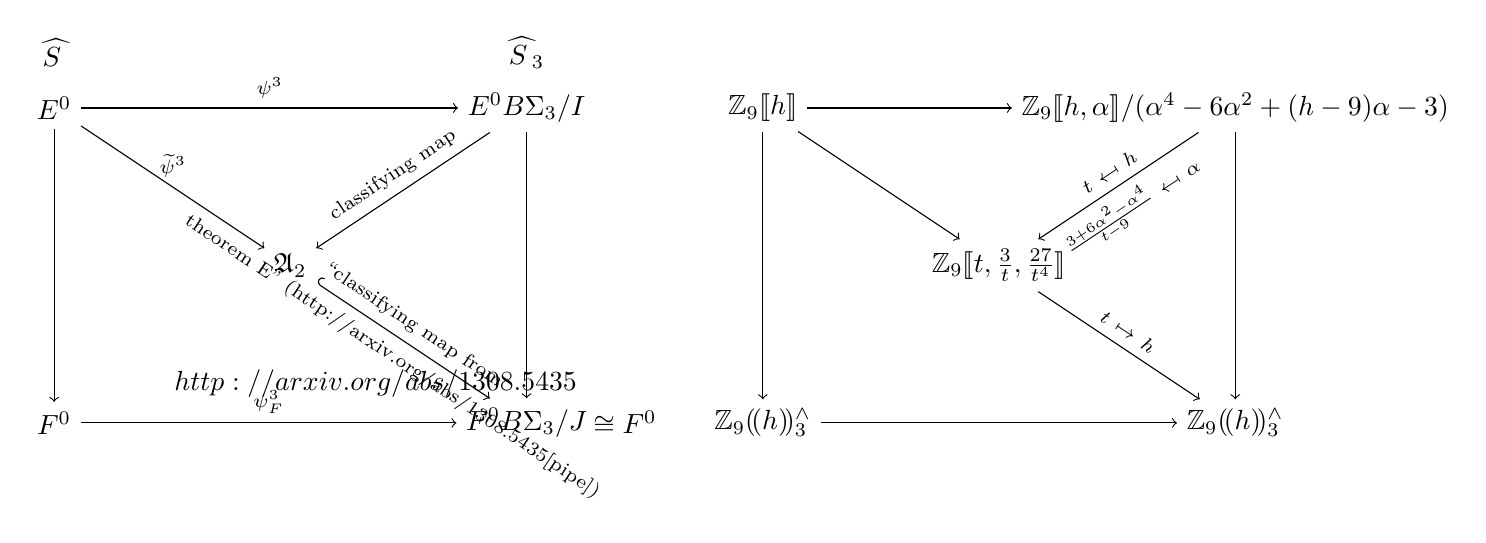
\begin{tikzpicture}[baseline=(current bounding box.center)]
         \node at (4.5, .5) {$\href{http://arxiv.org/abs/1308.5435}{\textcolor{white}{[pipe]}}$}; 
         \node (LT) at (0, 4) {$E^0$}; 
         \node at (0, 4.7) {$\HS$}; 
         \node (RT) at (6, 4) {$E^0 B\Sigma_3 / I$}; 
         \node at (6, 4.7) {$\HS_3$}; 
         \node (LB) at (0, 0) {$F^0$}; 
         \node (MB) at (6, 0) {$F^0 B\Sigma_3 / J$}; 
         \node (C) at (3, 2) {${\mf A_2}$}; 
         \node (RB) at (7.25, 0) {$\cong F^0$}; 
         \draw [->] (LT) -- node [above] {$\scriptstyle \p$} (RT); 
         \draw [->] (LT) -- (LB); 
         \draw [->] (RT) -- (MB); 
         \draw [->] (LB) -- node [above] {$\scriptstyle \psi_F^3$} (MB); 
         \draw [->] (LT) -- node [above] {$\scriptstyle \Tp^3$} (C); 
         \draw [->] (RT) -- node [above,sloped] {$\scriptstyle \text{classifying map}$} (C); 
         \draw [right hook->] (C) -- node [above,sloped] {$\scriptstyle \text{``classifying map from}$} 
                                     node [below,sloped] {$\scriptstyle \text{theorem E'' (\href{http://arxiv.org/abs/1308.5435}{[pipe]})}$} (MB); 
         \node (LT1) at (9, 4) {$\BZ_9 \lb h \rb$}; 
         \node (RT1) at (15, 4) {$\BZ_9 \lb h, \A \rb / (\A^4 - 6 \A^2 + (h - 9) \A - 3)$}; 
         \node (LB1) at (9, 0) {$\BZ_9 (\!( h )\!)^\wedge_3$}; 
         \node (MB1) at (15, 0) {$\BZ_9 (\!( h )\!)^\wedge_3$}; 
         \node (C1) at (12, 2) {$\BZ_9 \lb t, \frac{3}{t}, \frac{27}{t^4} \rb$}; 
         \draw [->] (LT1) -- (RT1); 
         \draw [->] (LT1) -- (LB1); 
         \draw [->] (RT1) -- (MB1); 
         \draw [->] (LB1) -- (MB1); 
         \draw [->] (LT1) -- (C1); 
         \draw [->] (RT1) -- node [above,sloped] {$\scriptstyle t ~\mapsfrom~ h$} 
                             node [below,sloped] {$\scriptstyle \frac{3 + 6 \A^2 - \A^4}{t - 9} ~\mapsfrom~ \A$} (C1); 
         \draw [->] (C1) -- node [above,sloped] {$\scriptstyle t ~\mapsto~ h$} (MB1); 
 \end{tikzpicture}
\end{equation}
where the map 
\[
 E^0 \to F^0 \xrightarrow{\psi^3_F} F^0 \qquad \text{lifts to} \qquad \Tp^3 \co E^0 \to \mf A_2 
\]
Computational evidence for $\psi^p_F(h) \in \mf A_2$ (in the absence of \href{http://tinyurl.com/jwtr2ba}{Atkin}): 
\begin{itemize}
 \item [p = 3] (\texttt{h1p3\_alpha\_h\_-20.nb}) We checked $\p_F(h)$ \eqref{h} down to $h^{-20}$ (first 24 terms): 
 the coefficients all contain sufficently many 3-factors, 
 precisely as many for the negative powers 1, 3, 5, 9, 13, 15, 17 of $h$; 
 the same conclusion (including those 7 specific negative powers) holds for $\A(h)$ down to $h^{-22}$.  

 \item [p = 2] (\texttt{2-K(1)\_a\_-52.nb}) We checked $\psi^2_F(a)$ down to $a^{-52}$ (first 19 terms): 
 \begin{equation*}
 \begin{split}
  \psi^2_F(a) = & ~ a^2 - 10 a^{-1} - 56 a^{-4} - 736 a^{-7} - 12288 a^{-10} - 230912 a^{-13} \\
                & - 4659200 a^{-16} - 98598912 a^{-19} - 2159149056 a^{-22} \\
                & - 46508277760 a^{-25} - 979219513344 a^{-28} - 20256129024000 a^{-31} \\
                & - 413760095256576 a^{-34} - 8374930945081344 a^{-37} \\
                & - 168325239044833280 a^{-40} - 3363201507053797376 a^{-43} \\
                & - 66848486735870951424 a^{-46} - 1322432066183409696768 a^{-49} \\
                & - 26047337841215500451840 a^{-52} \cdots 
 \end{split}
 \end{equation*}
 the coefficients all contain sufficently many 2-factors, 
 precisely as many for the negative powers 1, 4, 7, 13, 16, 28, 31, 34, 43, 49 of $a$; 
 the same conclusion (including those 10 specific negative powers) holds for $d(a)$ down to $a^{-52}$.  

 \item [p = 5] (\texttt{5-K(1)\_h\_-7.nb}) We checked $\psi^2_F(h)$ down to $h^{-7}$ (first 13 terms): 
 \begin{equation*}
 \begin{split}
  \psi^5_F(h) = & ~ h^5 - 10 h^4 - 1340 h^3 + 18440 h^2 + 267430 h - 3178250 \\
                & - 920120 h^{-1} + 183770000 h^{-2} - 11467367375 h^{-3} \\
                & + 449827523750 h^{-4} - 16654435175000 h^{-5} \\
                & + 595612985750000 h^{-6} - 21005686830531250 h^{-7} \cdots 
 \end{split}
 \end{equation*}
 the coefficients all contain sufficently many 5-factors, 
 precisely as many for the negative powers 3, 4, 5, 7 of $h$; 
 the same conclusion (including those 4 specific negative powers together with $-9$ and $-10$) holds for $\A(h)$ down to $h^{-11}$.  
\end{itemize}

Good things about $\mf A_2$: 
\begin{itemize}
 \item Has a uniform presentation for $p$ and $h$.  

 \item Is a classifying object.  

 \item Seems to be somewhere between height 1 and height 2.  
\end{itemize}

Questions: 
\begin{itemize}
 \item Would the ring $\mf A_h$ be something interesting in the context of $E$-\DL algebra?  

 \item Specifically, at height 2, could $\mf A_2$ be promoted as the target ring of a kind of ``canonical'' total power operation, 
 in the form 
 \begin{equation}
 \label{tt's}
  \BZ_{p^2} \llbracket t, t', s \rrbracket / (t t' - p, t^{p+1} s - \textcolor{red}{p^p}), 
 \end{equation}
 which descends to the {\em same} power operation $\p_F$ at height 1 as the total power operation $\p$?  
 How far is the classifying map $E^0 B\Sigma_3 / I \to {\mf A_2}$ in \eqref{A_2} from being an isomorphism?  
 It is injective.  

 Compare \eqref{tt's} with our known presentations for $E^0 B\Sigma_p / I$ [Sat-3/22/14, Tue-3/25/14]: 
 \begin{itemize}
  \item[-] $\textcolor{red}{p^p}$ shows up as the constant term in the degree-$(p+1)$ polynomial 
  satisfied by $\A'$---the parameter for the noncanonical subgroups / etale part, 
  possibly another ``deformation parameter'' along with the Hasse invariant 
  ($w(\A) \equiv \A (\A^p \pm h) \md p$, and $h \equiv \mp \A' \md \A$).  
  Thus the classifying map $E^0 B\Sigma_3 / I \to {\mf A_2}$ in \eqref{A_2} may be equivalently defined by 
  \[
   \A' \mapsto t 
  \]
  \[
   \A \mapsto -\frac{3}{t} 
  \]
  \[
   h = 9 - \A^3 + 6 \A - \A' \mapsto -t + 9 - \frac{18}{t} + \frac{27}{t^3} 
  \]
  For it to be surjective, we have the generator $\frac{27}{t^4}$ in 
  \[
   3^3 - 6 \cdot 3 \A'^2 - (h - 9) \A'^3 - \A'^4 = 0 
  \]
  that is, 
  \[
   \frac{27}{t^4} - 2 \A^2 - \frac{h - 9}{t} - 1 = 0 
  \]
  and in general there is always a term $\frac{h}{t}$ 
  so that the surjectivity needs $\A'$ to be genuinely inverted 
  (not just having $\frac{3}{\A'}$), ie ``canonical'' as opposed to ``universal.''  
  Is there a way to modify this generator and get an isomorphism?  

  \item[-] In \eqref{tt's} we have relations 
  \[
   t'^p = t s \qquad\qquad t'^{p+1} = p s 
  \]
 \end{itemize}

 \item Is $\mf A_2$ realizable?  
\end{itemize}


% \newpage
% \section{[level3]}
% \label{sec:level3}
% 
% - \textbf{Identifying the quantity we hope to be stable under the $K(1)$-local power operation $\psi$}
% 
% We have 
% \[
%  \pi_0 E_2 = {\mb Z}_9 \llbracket h \rrbracket,
% \]
% \[
%  \pi_0 L_{K(1)} E_2 = {\mb Z}_9 (\!(h)\!)_3^\wedge.
% \]
% We want to show that the subring
% \[
%  {\mb Z}_9 \left[\frac{v_2}{v_1^4}\right]_3^\wedge \subset \pi_0 L_{K(1)} E_2
% \]
% is stable under the power operation 
% \[
%  \psi\co \pi_0 L_{K(1)} E_2 \to \pi_0 L_{K(1)} E_2,
% \]
% where $|v_1| = 2(3^1-1) = 4$ and $|v_2| = 2(3^2-1) = 16$.  
% Note that as the generators of the homotopy of the generalized BP$\langle2\rangle$ spectrum, $v_1$ is only well-defined mod 3 and $v_2$ only mod $(3,v_1)$; 
% different choices of these congruence classes may correspond to {\em different} formal group laws the graded ring $\BZ_{(3)}[v_1,v_2]$ carries 
% (cf section 3 of [level3'] and [Fri-2/10/12]).
% 
% We need to make $v_2/v_1^4$ explicit. This amounts to a 3-primary analog of the last statement of proposition 5.4 on p29 of [level3] which is lemma 1 on p8 of [K(1)tmf]. 
% Explicitly, given the equation of our elliptic curve
% \[
%  C \co y^2 + a x y + a c y = x^3 + c x^2
% \]
% with $|a| = 2$, $|c| = 4$, and
% \[
%  a_1 = a, \quad a_2 = c, \quad a_3 = a c, \quad a_4 = a_6 = 0,
% \]
% we have, using the formula on p188 of [Pearson2], 
% 
% $m_0 = 1$,
% 
% $m_1 = \frac{1}{3} (a_2 + a_1^2) = \frac{1}{3} (c + a^2)$,
% 
% $m_2 = \frac{1}{9} (a_2^4 + 6 a_4^2 + 12 a_4 a_2^2 + 15 a_1^4 a_2^2 + 10 a_2^3 a_1^2 + 12 a_2 a_6 + 42 a_3 a_1^5 + 7 a_1^6 a_2 + 90 a_3^2 a_1^2
%  + 30 a_1^4 a_4 + 30 a_3^2 a_2 + 60 a_3 a_1 a_4 + 30 a_6 a_1^2 + 120 a_3 a_1^3 a_2 + 60 a_2^2 a_3 a_1 + 60 a_1^2 a_2 a_4 + a_1^8)
%  = \frac{1}{9} (c^4 + 100 c^3 a^2 + 225 c^2 a^4 + 49 c a^6 + a^8)$,
% 
% where $m_i$ is the coefficient of $x^{3^i}$ in $\log_C(x)$. Given the relations
% \[
%  3 m_1 = m_0 v_1, \quad 3 m_2 = m_0 v_2 + m_1 v_1^3,
% \]
% we then have
% \[
%  v_1 = c + a^2,
% \]
% \[
%  v_2 = 32 c^3 a^2 + 73 c^2 a^4 + 15 c a^6.
% \]
% \textcolor{red}{These use the coordinate $-x/y$ on $\HC$!  }
% 
% With the terminology in [level3'], our {\em (generalized) BP$\langle 2 \rangle$-realization problem} $(A,\BG)$ (definition 3.1 on p12) consists of
% \[
%  A = \BZ_{(3)}[v_1,v_2], \quad \BG = \widehat{C},
% \]
% and the {\em associated Lubin-Tate ring} (definition 4.1 on p19) is
% \[
%  B = \BZ_9 \llbracket u_1 \rrbracket [u^{\pm 1}].
% \]
% Writing
% \[
%  a = u t, \quad c = u^2, 
%  \footnote{Adjust so ``\textcolor{red}{+}'' below? Change the equation of $C$ below accordingly? Jacobi quartic (Ravenel? Edwards?): $y^2 = x^4 + A x^3 + C, |A| = 2, |C| = 8$.  }
% \]
% $C$ is isomorphic to
% \[
%  y^2 + t x y + t y = x^3 + x^2
% \]
% with $h = u_1 = t^2 + 4$. The $A$-algebra structure on $B$ is then given by
% \[
%  v_1 \mapsto u^2 (u_1 - 3) \equiv u_1 u^2 \md 3,
% \]
% \[
%  v_2 \mapsto u^8 (15 u_1^3 - 107 u_1^2 + 168 u_1 + 80) \equiv \textcolor{red}{-}\footnote{[Morava1207, 3.5]?}u^8 \md (3, u_1 u^2)
% \]
% ({\em Is this reasonable?}).\\
% 
% \hrule
% 
% - (\texttt{h1p3\_alpha\_H\_-2.nb} and \texttt{closure.nb}) \textbf{Calculating $\psi(v_2 / v_1^4)$}
% 
% From above we have
% \begin{eqnarray*}
%  \frac{v_2}{v_1^4} & = & \frac{32 c^3 a^2 + 73 c^2 a^4 + 15 c a^6}{(c + a^2)^4} \\
%                    & = & \frac{32 t^2 + 73 t^4 + 15 t^6}{(1 + t^2)^4} \\
%                    & = & \frac{32 (h - 4) + 73 (h - 4)^2 + 15 (h - 4)^3}{(h - 3)^4} \\
%                    & = & \frac{15}{H} + \frac{\textcolor{blue}{28}}{H^2} - \frac{69}{H^3} + \frac{\textcolor{blue}{26}}{H^4},
% \end{eqnarray*}
% where $H = h -3$. We then compute that
% \[
%  \psi(H) = H^3 - 27 H^2 + 183 H - 180 + \frac{186}{H} + \frac{1674}{H^2} + \cdots,
% \]
% and solve that
% \[
%  \psi(\frac{1}{H}) = \frac{1}{H^3} + \frac{27}{H^4} + \frac{546}{H^5} + \frac{9981}{H^6} + \frac{174243}{H^7} + \frac{2969622}{H^8} + \cdots,
% \]
% and thus
% \[
%  \psi(\frac{v_2}{v_1^4}) = \frac{15}{H^3} + \frac{405}{H^4} + \frac{8190}{H^5} + \frac{\textcolor{blue}{149743}}{H^6} + \frac{2615157}{H^7} + \frac{44595318}{H^8} + \cdots.
% \]
% Comparing the formulas of $v_2 / v_1^4$ and $\psi(v_2 / v_1^4)$, we conclude that the subring ${\mb Z}_9 [v_2 / v_1^4]_3^\wedge$ is not stable under $\psi$, 
% as 15 is not invertible in $\BZ_9$ (the leading terms should match; cf 2/13/12 email).\\
% 
% \hrule
% 
% \textbf{Problem?} [6/20/13 email] 
% \[
% A = \BZ_{(3)} [a,c], \qquad \BG = \HC 
% \]
% but $A / (3,v_1,v_2) \not\cong \BF_3$ contradicts [level3', def 3.1].  
% 
% \textbf{Understand} what [level3] and [level3'] are doing.  
% {\em There are more details to be worked out and it's not quite as straightforward as I may have hoped when writing level3, 
% but I feel like it should be possible to figure out a lot about what kinds of schemes would have to carry p-divisible groups in order to make Jacob's machine work.  }
% 
% Perhaps the $\G_1(4)$ curve gives a non-example, and some other curve (Jacobi quartic?) gives an example, at the prime 3.  
% {\em It seems unclear whether there is some 
% isomorphism from this formal group law on $A$ to one coming from the 
% smaller subring $\BZ_{(p)}[v_1,v_2] \subset A$ which has reasonable isogeny 
% properties.  The same is true for most of the other modular curves.}  
% 
% So the machine in [level3] needs nice input data of specific formal group laws to work, 
% even if we have some explicit calculations of power operations on Lubin-Tate spectra of height 2 at the prime 3.  
% The paper [logetaletmf] should solve this realization problem in general (see the ``hope'' recorded on [level3, pp4-5]).  
% 
% 
% \newpage
\section{\href{http://arxiv.org/abs/math/0407022}{[log]}}

\begin{itemize}
 \item Clarify the relationship between topological and classical Hecke operators.  

 \item Kernel of the logarithm.  
\end{itemize}


% \texttt{It is notable that this expression from the theory of $L$-functions arises naturally from a purely topological construction; 
% it came as a surprise to the author, 
% and he still has no good explanation for it.  
% It is also significant for the application to elliptic cohomology; 
% in the presence of an elliptic curve, 
% these Hecke operators coincide with the classical action of Hecke operators on modular forms.  }
% 
% MF$(\BZ) = \BZ [c_4, c_6, \Delta, \Delta^{-1}] / (c_4^3 - c_6^2 = 1728 \Delta)$ 
% 
% \texttt{The key tool here is Rezk's $K(1)$-local logarithm, which permits a $K(1)$-local analysis of $Pic(Sp)$.  }


\subsection{Logarithms}

$l_{2,p} \co (E^0)^\times \to E^0$ 

$l_{2,p}(x) = \sum_{k=1}^\infty (-1)^{k-1} \frac{p^{k-1}}{k} M(x)^k = \frac{1}{p} \log(1 + p M(x))$ 

\begin{equation*}
\begin{split}
 1 + p M(x) = & ~ \prod_{j=0}^2 \prod_{\text{subgroups $A$ of order $p^j$}} \psi_A(x)^{(-1)^j p^{(j-1)(j-2)/2}} \\
            = & ~ x^p \cdot \frac{1}{\psi^p(x;\A_1) \cdots \psi^p(x;\A_{p+1})} \cdot \Psi(x) \\
            = & ~ \frac{x^{p+1}}{\psi^p(x;\A_1) \cdots \psi^p(x;\A_{p+1})} \qquad\qquad\qquad\qquad \text{multiplicative, not additive, sends scalars to 1} 
\end{split}
\end{equation*}

Question: How to interpret $M$ in AT and in NT (cf the values of $M$ in p = 2, p = 3, and h = 1 below)?  


\subsection{p = 2 (\texttt{log2.nb})}

$E^0 = \BZ_4 \lb a \rb$ 

$y^2 + a x y + y = x^3$ 

$\Delta = a^3 - 27 = (a - 3) (a^2 + 3 a + 9) \in (E^0)^\times$ 

$c_4 = a^4 - 24 a = a (a^3 - 24)$ 

$c_6 = -a^6 + 36 a^3 - 216$ 

\[
 1 + 2 M(\Delta) = -1 \implies M(\Delta) = -1, \quad l_{2,2}(\Delta) = 0 
\]
\[
 1 + 2 M(a - 3) = -1 \implies M(a - 3) = -1, \quad l_{2,2}(a - 3) = 0 
\]
\[
 \implies 1 + 2 M(a^2 + 3 a + 9) = 1 \implies M(a^2 + 3 a + 9) = 0, \quad l_{2,2}(a^2 + 3 a + 9) = 0 
\]
These factors exhaust all linear, quadratic, cubic, and quartic polynomials in $\ker l_{2,2}$.  

Moreover, 
\[
 1 + 2 M(c_4) = \frac{a^3 (a^3 - 24)^3}{(a^3 - 54) (a^9 - 18 a^6 + 756 a^3 - 27000)} \implies M(c_4) = \frac{27000 \Delta}{c_4^3 - 2 \cdot 27000 \Delta} = \frac{27000}{j - 54000} 
\]
\[
 1 + 2 M(a) = -\frac{a^3}{a^3 - 54} \implies M(a) = \frac{\Delta}{27 - \Delta} 
\]
\[
 \implies 1 + 2 M(a^3 - 24) = -\frac{(a^3 - 24)^3}{a^9 - 18 a^6 + 756 a^3 - 27000} 
\]
\[
 \qquad \qquad \qquad \qquad \qquad M(a^3 - 24) = -\frac{\Delta ((a^3 - 24)^3 - 27000)}{c_4^3 - 2 \cdot 27000 \Delta} = \dfrac{27000 - (a^3 - 24)^3}{j - 2 \cdot 27000} 
\]
and 
\[
 1 + 2 M(c_6) = \frac{(a^6 - 36 a^3 + 216)^2}{a^{12} - 72 a^9 + 1728 a^6 -301320 a^3 + 7762392} 
 \implies M(c_6) = \frac{142884 \Delta}{c_6^2 - 2 \cdot 142884 \Delta} = \frac{142884}{j - 287496} 
\]


\subsection{p = 3 (\texttt{log3.nb})}

$E^0 = \BZ_9 \lb h = a^2 + 1 \rb$ 

$y^2 + a x y + a y = x^3 + x^2$ 

$\Delta = a^2 (a + 4) (a - 4) = (h - 1) (h - 17) = h^2 - 18 h + 17 \in (E^0)^\times$ 

$c_4 = a^4 - 16 a^2 + 16 = h^2 - 18 h + 33$ 

$c_6 = -(a^2 - 8) (a^4 - 16 a^2 - 8) = -(h - 9) (h^2 - 18 h + 9) = -h^3 + 27 h^2 - 171 h + 81$ 

\[
 1 + 3 M(a) = 1 = 1 + 3 M(a \pm 4) \implies M(a) = M(a \pm 4) = M(\Delta) = 0 = l_{2,3}(\Delta) = l_{2,3}(a \pm 4) = l_{2,3}(a) 
\]
but 
\[
 1 + 3 M(h) = \frac{h^4}{h^4 + 153 h^3 - 7395 h^2 + 86139 h - 78897} \implies M(h) = \frac{-17 \Delta (3 h - 91)}{\cdots} 
\]
\[
 1 + 3 M(3 h - 91) = \frac{(3 h - 91)^4}{81 h^4 - 685668 h^3 + 12612294 h^2 - 20532132 h + 68574961} \implies M(3 h - 91) = \frac{225280 \Delta h}{\cdots} 
\]

Moreover, 
\[
 M(c_4) = -\frac{4096000 \Delta}{c_6^2 + 12289728 \Delta} = -\frac{4096000}{j + 3 \cdot 4096000} 
\]
and 
\[
 1 + 3 M(h - 9) = \frac{(h - 9)^4}{h^4 - 36 h^3 + 12774 h^2 - 224100 h + 215457} \implies M(h - 9) = -\frac{4096 \Delta}{(c_4 + 12384) c_4 - 194304} 
\]
\[
 1 + 3 M(h^2 - 18 h + 9) = \cdots \implies M(h^2 - 18 h + 9) = \frac{4096 \Delta ((c_4 + 15) c_4 + 12000)}{(((c_4 - 12384) c_4 + 15744) c_4 - 144562176) c_4 + 2359627776} 
\]
\[
 \implies 1 + 3 M(c_6) = (1 + 3 M(h - 9)) (1 + 3 M(h^2 - 18 h + 9)) \implies M(c_6) = \frac{602112 \Delta (85 c_6^2 + 1138368 \Delta)}{K} 
\]
with 
\begin{equation*}
\begin{split}
    K = & ~ ((((c_4^2 - 153542016) c_4 + 2456672256 ) c_4 - 1790957481984) c_4 + 57310639423488) c_4 - 458485115387904 \\
 \equiv & ~ c_4^6 \md 3 
\end{split}
\end{equation*}


\subsection{h = 1 (\texttt{2-K(1).nb})}

$l_{1,p} \co (F^0)^\times \to F^0, x \mapsto \frac{1}{p} \log(1 + p M(x))$ 

$1 + p M(x) = \dfrac{x^p}{\psi^p(x)}$ 

When $p = 2$, $F^0 = \BZ_4 \lp a \rp_2^\wedge$ and 
\[
 \psi^2(a) = a^2 - 10 a^{-1} - 56 a^{-4} - 736 a^{-7} - 12288 a^{-10} + \cdots 
\]
\[
 \implies 1 + 2 M(a) = 1 + 10 a^{-3} + 156 a^{-6} + 2856 a^{-9} + 56944 a^{-12} + \cdots 
\]
When $p = 3$, $F^0 = \BZ_9 \lp h \rp_3^\wedge$ and 
\[
 \p(h) = h^3 - 27 h^2 + 183 h - 180 + 186 h^{-1} + 1674 h^{-2} + 13878 h^{-3} + \cdots 
\]
\[
 \implies 1 + 3 M(h) = 1 + 27 h^{-1} + 546 h^{-2} + 9981 h^{-3} + 174243 h^{-4} + \cdots 
\]
Question: Is $l_{1,p}$ surjective as in \href{http://arxiv.org/abs/1110.5851}{[Clausen, proposition 4.1]}?  Unlikely.  


\subsection{h = 2, Hecke operators}

[4/22/14 email]: At height 2, $\Delta$ and its factors seem to always be in the kernel of $l_{2,p} \co (E^0)^\times \to E^0$.  

\underline{Proof} of $\Delta \in \ker l_{2,p}$ \\
As observed in [log, 1.12], 
\[
 l_{n,p}(x) = F_1(\log x); 
\]
when $n = 2$, 
\[
 F_1 = 1 - T_p + (T_p T_p - T_{p^2}).  
\]
\href{http://galoisrepresentations.wordpress.com/2012/10/26/jacobi-by-pure-thought/}{The logarithmic derivative $f$ of $\Delta$} 
is the quasi-modular Eisenstein series $E_2$; 
it is a weight 2 eigenform for every $T_m$ with eigenvalue $\sigma_1(m)$.  
Thus one computes that $F_1 \thinspace f = 0$.  
Since the action of Hecke operators commutes with taking derivatives 
(see proposition 4 \href{http://arxiv.org/abs/math/0610861}{here} and the end of section 5 of \href{http://arxiv.org/abs/1205.2408}{this}), 
this implies that $(F_1 \log \Delta)' = 0$ and so 
\[
 l_{2,p}(\Delta) = F_1 \log \Delta = \text{some constant}~ c(p).  
\]
Using Rezk's work (or an analogous calculation at $p = 3$) one computes that $c(2) = 0$.  
Thus for a general prime, 
\[
 c(p) = F_{1,p}(\log \Delta) = \frac{2}{3} \thinspace F_{1,2} \thinspace F_{1,p}(\log \Delta) 
 = \frac{2}{3} \thinspace F_{1,p} \thinspace F_{1,2}(\log \Delta) 
 = \frac{2}{3} \thinspace F_{1,p}(0) = 0.  
\]

% \texttt{The $K(2)$-local logarithm should certainly have a kernel - 
% the chromatic pullback square for the $(K(1) \vee K(2))$-localization of $gl_1 E$ 
% involves not only the $K(2)$-local logarithm, but also the $K(1)$-local logarithm.  
% Put together, the ``complete'' kernel for this should be zero in high degrees due to Ando-Hopkins-Rezk, Thm 4.11.  }
% 
% \texttt{The kernel of the $K(2)$-local logarithm consisted of forms that satisfied a relation satisfied by the Eisenstein series 
% (which are Hecke eigenforms themselves, but pretty far distinct from the discriminant).  
% Then, on this kernel, you had something approaching the Atkin operator acting coming from the remaining $K(1)$-local logarithm material.  }

Question \href{http://arxiv.org/abs/0812.1320}{[h2p2, exe 2.9]}: What is $\ker l_{2,p}$?  
Look into \href{http://www.math.uiuc.edu/~mando/papers/koandtmf.pdf}{[koandtmf]} and Serre's formes modulaires p-adiques paper.  \\%See also \eqref{log}.  

\hrule

Write $\tilde{T}_p = \sum_{\text{subgroups} ~ A ~ \text{of order} ~ p} \psi_A$ 
\begin{itemize}
 \item [p = 2]

 $\Delta = a^3 - 27$ \hfill $h = a$ 

 $c_4 = a^4 - 24 a = a (a^3 - 24)$ 

 $c_6 = -a^6 + 36 a^3 - 216$ 

 $\tilde{T}_2(\Delta) = \Delta (a^3 - 3)$ \hfill $\tau(2) = \textcolor{red}{-}24$ 

 \hfill $a^3 - 3 = 24 \implies a = 3$ 

 $\tilde{T}_2(c_4) = a^2 (354 - 40 a^3 + a^6)$ \hfill $\sigma_3(2) = 9$ 

 \hfill $a (354 - 40 a^3 + a^6) = 9 \implies a = 3$ 

 \hfill $c_4(3) = 9, \tilde{T}_2(c_4)(3) = 27$ 

 $\tilde{T}_2(c_6) = -3564 + 6534 a^3 - 1128 a^6 + 60 a^9 - a^{12}$ \hfill $\sigma_5(2) = 33$ 

 \hfill $c_6(3) = 27, \tilde{T}_2(c_6)(3) = 81$ 

 \item [p = 3]

 $\Delta = h^2 - 18 h + 17$ 

 $c_4 = h^2 - 18 h + 33$ 

 $c_6 = -h^3 + 27 h^2 - 171 h + 81 = -(h - 9) (h^2 - 18 h + 9)$ 

 $\tilde{T}_3(\Delta) = \Delta (2413 - 1908 h + 430 h^2 - 36 h^3 + h^4)$ \hfill $\tau(3) = 252$ 

 \hfill $2413 - 1908 h + 430 h^2 - 36 h^3 + h^4 = \textcolor{red}{-}252 \implies h = 5 ~\text{or}~ h = 13$ 

 \hfill $\Delta(5) = \Delta(13) = -48$ 

 $\tilde{T}_3(c_4) = c_4 (1245 - 1620 h + 414 h^2 - 36 h^3 + h^4)$ \hfill $\sigma_3(3) = 28$ 

 \hfill $c_4(5) = c_4(13) = -32, \tilde{T}_3(c_4)(5) = \tilde{T}_3(c_4)(13) = (-32) (-380)$ 

 $\tilde{T}_3(c_6) = -(h - 9) (921351 - 2452032 h + 2399040 h^2 - 1091232 h^3 + 251928 h^4 - 31104 h^5 + 2088 h^6 - 72 h^7 + h^8)$ \hfill $\sigma_5(3) = 244$ 

 \hfill $c_6(5) = -224, \tilde{T}_3(c_6)(5) = -224 \cdot 2164$ 

 \hfill $c_6(13) = 224, \tilde{T}_3(c_6)(13) = 224 \cdot 2164$ 

 \textcolor{gray}{($\tilde{T}_3(h^2 - 18 h + 16) = 41017 - 75870 h + 44067 h^2 - 10260 h^3 + 1095 h^4 - 54 h^5 + h^6$) }
\end{itemize}
Question [\texttt{eigen.nb}]: 
\begin{itemize}
 \item[] How to address $\Delta$, $c_4 = (2 \pi)^4 E_4$, $c_6 = (2 \pi)^6 E_6$ not being eigenforms of $\tilde{T}_p = \sum \psi_A$ 
 (with eigenvalues $\tau(p)$, $\sigma_3(p)$, $\sigma_5(p)$ respectively)?  

 \item[] How to address the weight?  Why do Hecke operators preserve weight?  

 \item[] Perhaps the weight discrepancy has to do with $\psi_A$ being computed from a universal example.  

 \item[] Perhaps we should have taken into account the $\G_1(N)$ structure.  
\end{itemize}

All of these seem to have made an appearance in \href{http://tinyurl.com/qdtdpaw}{[K(1)E$_\infty$]}; revisit and put these in context.  


% \newpage
% \section{Functoriality}
% 
% {\em The structure of power operations: Witt vectors, plethories}
% 
% (\texttt{6/1 email: Witt vectors}) \textbf{Ideas}
% 
% - Calculational approach (Hazewinkel, Pearson, ...)
% 
% There is a formula-based approach to the ``generalized'' Witt ring. 
% It is section 25.1 ``The Witt-vector-like group functor $W^F$ attached to a one dimensional formal group law $F(X, Y)$'' of FG, notably theorem 25.1.12 and remark 25.1.14 on pp270-1.
% 
% Hazewinkel's formulas for the functor $W^F$ may allow us to compute explicitly. 
% When $F$ is the additive formal group law, we may get something showing up in the mod-$p$ Steenrod algebra structure ({\em Check!}). 
% When $F$ is the formal group law for a specific elliptic curve, hopefully we may be able to recover some of the formulas in [h2p2] and [p3].
% 
% The idea is that there might be a connection:
% 
% ~~~~~~~~ power operations $\leftrightsquigarrow$ structure of subgroups
% 
% ~~~~~~~~~~~~~~~~~~~~~~~~~~~~~~~~~~~~~~~~~~~~~~~~ formal group law $\leftrightsquigarrow$ Witt vectors
% 
% {\em Anything in the literature about Witt vectors capturing structure of subgroups?}
% 
% \begin{itemize}
% \item Dieudonn\'e modules (\url{http://en.wikipedia.org/wiki/Group_scheme#Dieudonn.C3.A9_modules} and the main article from there 
% \footnote{A readable introduction to the theory of Dieudonn\'e modules might be (the first three chapters of) {\em Groupes $p$-divisibles sur les corps locaux} by Jean-Marc Fontaine.  }):
% 
% Finite flat commutative group schemes over a perfect field $k$ of positive characteristic $p$ 
% can be studied by transferring their geometric structure to a (semi-)linear-algebraic setting. 
% The basic object is the Dieudonn\'e ring $D = W(k)\{F,V\}/(FV - p)$, 
% which is a quotient of the ring of noncommutative polynomials, 
% with coefficients in Witt vectors of $k$. 
% $F$ and $V$ are the Frobenius and Verschiebung operators, 
% and they may act nontrivially on the Witt vectors. 
% Dieudonn\'e and Cartier constructed an antiequivalence of categories 
% between finite commutative group schemes over $k$ of order a power of $p$ 
% and modules over $D$ with finite $W(k)$-length. 
% The Dieudonn\'e module functor in one direction is given by homomorphisms into the abelian sheaf $CW$ of Witt co-vectors. 
% This sheaf is more or less dual to the sheaf of Witt vectors (which is in fact representable by a group scheme), 
% since it is constructed by taking a direct limit of finite length Witt vectors under successive Verschiebung maps $V\co W_n \to W_{n+1}$, and then completing.
% 
% Grothendieck suggested that there should be a crystalline version of the theory that could be used to analyze $p$-divisible groups.
% 
% \item Ando's notes on Dieudonn\'e crystals may be relevant, especially to the last point above.
% 
% \item Chapter V, in particular section 27, of FG. Cf question \eqref{curves}.
% 
% \item So the power operations may be an algebra over the Dieudonn\'e ring (rather than simply the ring itself), which might then involve $\alpha$ as a generator? 
% (\texttt{Do you feel like you could define Witt vectors of length two given the quantity `$d$'? Do you need higher information to define Witt vectors of higher length?})
% 
% This may be a continuation of ideas of Goerss, Pearson, ... (see note to [Pearson1] below):
% 
% {\em The category of graded, bicommutative Hopf algebras over the
% prime field with $p$ elements is an abelian category which is equivalent, by work
% of Schoeller, to a category of graded modules, known as Dieudonn\'e modules.
% Graded ring objects in Hopf algebras are called Hopf rings, and they arise
% in the study of unstable cohomology operations for extraordinary cohomology
% theories. The central point of this paper is that Hopf rings can be studied by
% looking at the associated ring object in Dieudonn\'e modules. They can also be
% computed there,} ...
% 
% \item Given the relationship between the Dieudonn\'e ring and the Morava stabilizer group (the automorphism group of the formal group law we are concerned with), 
% we might try to consider if there is a higher chromatic analog of the dual Steenrod algebra being the automorphism group scheme of the formal additive group 
% (\url{http://mathoverflow.net/questions/83096/is-there-a-high-concept-explanation-of-the-dual-steenrod-algebra-as-the-automorph})? 
% Cf p44 and pp22-4 (including the $K$-theory calculations) of [coctalos].
% 
% \item However, the Witt ring involved in the usual Dieudonn\'e modules is for the multiplicative formal group law, 
% but we want to study the Witt ring for the formal group law which we are interested in. 
% So perhaps we need the corresponding ``generalized'' Dieudonn\'e modules? We want functoriality.
% \end{itemize}
% 
% - Conceptual approach (Borger-Wieland, Strickland, ...)
% 
% For the Borger-Wieland approach, according to Rezk's terminology of calling the homotopy of a $K(n)$-local commutative $E$-algebra a graded amplified $\Gamma$-ring, 
% the ring $\Gamma$ of power operations might be the additive bialgebra of an $E_0$-plethory (corresponding to $\mb T$) in the sense of Borger-Wieland 
% (cf 1.8 on p253 of their published paper). They construct conceptually (formula-free) a $\mb Z$-plethory $\Lambda_p$ by a process of amplification 
% (reminiscent of deformation of Frobenius), and the ring of Witt vectors ({\em comparable to the homotopy acted on by the power operations?}) 
% ``is simply the $\Lambda_p$-ring co-induced from the ring $R$''. The construction is carried out in section 12 
% (especially 12.1, quite echoing ``Frobenius producing power operations''), and the notion of amplification is explained in section 7 (there is a universal object, cf theorem 7.1). 
% We might be able to carry out a similar procedure and construct structures relevant to power operations for Morava $E$-theory (at least conceptually).
% 
% The hope is that, given the functoriality of this construction, we might then be able to get useful information from one $E$-theory to another, 
% or get more information on one $E$-theory through self-maps, combining the calculational results we might have from the previous approach 
% which might also be functorial (say a natural transformation $W^F \to W^G$).
% 
% The first half of section 7 (Tambara functors) of Strickland's list and the references mentioned there ([1,3,5,9]) might also be relevant, in particular the preprint [9]. 
% Also Morten Brun has two more papers ``Witt vectors and equivariant ring spectra'' and ``Witt vectors and equivariant ring spectra applied to cobordism''.
% 
% Tambara functors {\em encode the algebraic structure of the zeroth homotopy group of an equivariant, strictly commutative ring spectrum}. 
% {\em Tambara functors are to rings what Mackey functors are to abelian groups.} 
% ... {\em a link between Witt rings (in the generalised sense of Dress and Siebeneicher) and free Tambara functors} ... 
% {\em These Witt rings (for cyclic groups of equivariance) are related to topology in two different ways. 
% On the one hand, for any ($-1$)-connected strictly commutative ring spectrum $A$, there is a topological Hochschild homology spectrum $THH(A)$ with a circle action, 
% whose equivariant homotopy groups in degree zero can be described in terms of Witt rings. 
% On the other hand, if we fix a prime $p$, we can fit together Witt rings in a certain way to form a ``Dieudonn\'e module'' for any bicommutative Hopf algebra over $\mb Z/p$. 
% Paul Goerss has shown that this construction is relevant to the generalised homology of the important space $\Omega^2 S^3$} ...
% 
% N.P. Strickland, Functorial philosophy for formal phenomena, in preparation. (See the introduction and section 14 of [Str97] for what might be in there.)
% \\
% 
% \hrule
% 
% \subsection{(Re)visiting [cong] and [h2p2]}
% 
% \subsubsection{[cong]}
% 
% \S 1: from conceptual to calculational
% \begin{itemize}
%  \item (1.1) Power operation structure in terms of $\mb T$.
% 
%  \item (1.2) Power operation structure in terms of $\Gamma$: connected to $\mb T$ via theorem A.
% 
%  \item (1.4) Power operation structure in terms of formal groups and Frobenius isogenies: basis for calculations (theorem B); work of Ando, Hopkins, Strickland, ... (1.5).
% \end{itemize}
% Q:
% \begin{enumerate}
%  \item In (1.7), precisely what are the ``completion issues'' (cf ${\mb T}(\pi_* M) \approx [\pi_* {\mb P} M]_{\mf m}^\wedge$ in (3) on top of p2)? 
%  Related to ``optimal deformation theory'' (cf 5/26 email)?
% \end{enumerate}
% 
% \S 2: grading
% \begin{itemize}
%  \item (2.10) The twisted ${\mb Z}/2$-graded tensor category ${\rm Mod}_{E_0}^*$: twisted by $\omega = \pi_2 E$.
% \end{itemize}
% 
% \S\S 3 (preliminaries), 4 (main constructions and properties): the monad $\mb T$ (Dyer-Lashof theory)
% \begin{itemize}
%  \item (3.3, 3.4(3)) The completion functor: $K(n)$-localization of (finite free) $E$-modules.
% 
%  \item (3.15) Completed extended powers: homotopy category, completion issues for ${\mb P}(-)$.
% 
%  \item (3.23) Construction of power operations (in terms of $\mb P$): 
%  including a relative version (3.26) and (as its application) power operations in non-zero degrees (3.27).
% 
%  \item (4.4) Construction of the {\em algebraic approximation functors} ${\mb T}_m$ and $\mb T$: 
%  for a finite free $E_*$-module $M_*$, define ${\mb T}_m (M_*) = \pi_* L {\mb P}_m (M)$; 
%  then extend to all $E_*$-modules by left Kan extension.
% 
%  \item (4.6) Construction of the {\em algebraic approximation map} $\alpha \co {\mb T} (\pi_* M) \to \pi_* L {\mb P} (M)$: 
%  $\alpha_m \co {\mb T}_m (\pi_* M) \to \pi_* L {\mb P}_m (M)$ are isomorphisms on finite free $E$-modules, basically constructed from definition of ${\mb T}_m$.
% 
%  \item Structure of ${\mb T} \co {\rm Mod}_{E_*} \to {\rm Mod}_{E_*}$:
% 
%  - (4.10, 3.16) it admits the structure of a {\em monad} (compatible with the monad structure of $L{\mb P} \co h{\rm Mod}_E \to h{\rm Mod}_E$);
%  
%  - (4.15) it admits the structure of a {\em symmetric monoidal functor} $({\rm Mod}_{E_*}, 0, \oplus) \to ({\rm Mod}_{E_*}, E_*, \otimes)$;
% 
%  - (4.24) it admits a {\em weight decomposition} compatible with the monad and (strictly graded, see (3.22)) commutative ring structures on $\mb T$;
% 
%  - (4.22) the forgetful functor $U \co {\rm Alg}_{\mb T}^* \to {\rm Alg}_{E_*}$ is {\em plethyistic}, 
%  so that the category of $\mb T$-algebras ${\rm Alg}_{\mb T}^*$ is equivalent to the categories of $M = UF$-algebras and $C = UG$-coalgebras (Beck's theorem, p151 of CT).
% 
%  \item Variants of $\mb T$: homotopy category $\widetilde{\mb T}_m \co h{\rm Mod}_E \to {\rm Mod}_{E_*}$ (4.6); 
%  completion $\widehat{\mb T} = L_0 {\mb T}$ (4.16).
% 
%  \item (4.20) Reconstruction of (completed) power operations in terms of $\mb T$ (via ${\mb T}_m (M_*) = \pi_* L {\mb P}_m (M)$), including in non-zero degrees (4.25).
% \end{itemize}
% Q:
% \begin{enumerate}
%  \item Last part of the proof of (4.23) related to ``generalized Witt vectors''? 
%  (Yes, see \url{http://mathoverflow.net/questions/58/is-there-a-universal-property-for-witt-vectors/89#89}, and cf (E.2.2) on p145 of FG.)
% \end{enumerate}
% 
% \S\S 5 (general), 6 (specific), 7 (non-zero degrees): the twisted bialgebra $\Gamma$ (Dyer-Lashof algebra)
% \begin{itemize}
%  \item (5.3) {\em Twisted cocommutative $R$-bialgebra} $(\Gamma, \epsilon, \Delta, \eta, \mu)$: $\Gamma$ and its ``manifest'' $H_\Gamma \co {\rm Mod}_R \to {\rm Mod}_R$ which 
%  (cf structure of ${\mb T} \co {\rm Mod}_{E_*} \to {\rm Mod}_{E_*}$ in \S 4)
% 
%  - admits the structure of a {\em comonad} (cf the comonad $C = UG$ in (4.22)),
% 
%  - admits the structure of a {\em symmetric monoidal functor},
% 
%  - (5.7) admits a {\em grading} which gives rise to an {\em affine graded category scheme} ${\cal A} = (R, A[k] \coloneqq H_{\Gamma [k]}(R), s^*, t^*, i^*, c^*)$,
% 
%  - (5.6) the forgetful functor $U \co {\rm Alg}_{\Gamma} \to {\rm Alg}_R$ is {\em plethyistic}.
% 
%  \item (5.8) $\Gamma$-modules (5.3) can be described more concretely as $\cal A$-comodules.
% 
%  \item (6.2) Construction of $\Gamma$ (the algebra of additive operations on $\pi_0$ of a $K(n)$-local commutative $E$-algebra spectrum): 
%  ${\mb T}_m (E_*) \cong E_*^\wedge B\Sigma_m$ (link to topology), RHS computed in [Str98], 
%  $\Gamma[k] \subset {\mb T}_{p^k} (E_0)$ defined by modulo the transfer ideal (be careful about homology/cohomology), 
%  finite free as an $E_0$-module (6.3).
% 
%  \item (6.5) Example of $\Gamma$ for $p$-adic $K$-theory: $\Gamma \cong {\mb W}k \langle \psi^p \rangle$.
% 
%  \item (6.6) Construction of $\omega$ (a symmetric object in ${\rm Mod}_\Gamma$ taking care of odd degrees): 
%  $\omega = {\rm ker}_{{\rm Alg}_\Gamma} (E^0({\mb CP}^1) \to E^0)$ (cf p8 of [h2p2], and compare the definition of a complex orientation of $E$).
% 
%  \item (7.1) Construction of $\Gamma^q$ (acting on $\pi_{-q} A$): generalizes (6.2) for $\Gamma = \Gamma^0$.
% 
%  \item (7.5) Relationship among different degrees $q$ in terms of the primitives and indecomposables of $\pi_q L {\mb P}_{p^k} \Sigma^q E$: 
%  {\em the present paper is essentially a meditation on} ${\rm coker} ({\rm Prim}_0 \rightarrowtail \pi_0 L {\mb P}_{p^k} E \twoheadrightarrow {\rm Ind}_0)$.
% 
%  \item (7.9) The $\mb Z$-graded category ${\rm Mod}_{\Gamma^*}^{\mb Z *}$ and its ``strengthened'' version ${\rm Mod}_{\widetilde{U}^* E_*}^{\mb Z *}$.
% 
%  \item (7.10-) Reformulate ${\rm Mod}_{\widetilde{U}^* E_*}^{\mb Z *}$ in terms of $\Gamma$ by defining the $\omega$-twisted ${\mb Z}/2$-graded category 
%  ${\rm Mod}_\Gamma^*$ equivalent to ${\rm Mod}_{\widetilde{U}^* E_*}^{\mb Z *}$ (7.23), 
%  using the periodicity of $E_*$ (7.11) and the suspension isomorphism $\Gamma^1 \to \Gamma^0$ (7.17) (cf (7.5)), 
%  such that the forgetful functor $U \co {\rm Alg}_{\mb T}^* \to {\rm Alg}_\Gamma^*$ is plethyistic (cf (5.6) and (4.22)).
% \end{itemize}
% Q:
% \begin{enumerate}
%  \item ``Bialgebras can be thought of as a kind of `dual' version of the notion of Hopf algebroids'' ((5.0), (5.8)) specializes to the dual Steenrod algebra?
% 
%  \item Proof of (7.3)? And results in [Str98]...
% 
%  \item What precisely is the relationship between ${\rm Mod}_{\Gamma^*}^{\mb Z *}$ and ${\rm Mod}_{\widetilde{U}^* E_*}^{\mb Z *}$? 
%  Why do we want the latter? So as to make the forgetful functor $\widetilde{U}^* \co {\rm Alg}_{\mb T}^* \to {\rm Mod}_{\widetilde{U}^* E_*}^{\mb Z *}$ 
%  {\em strong} symmetric monoidal? Related to theorem A?
% \end{enumerate}
% 
% \S\S 8 (rational objects), 9 (regular weights), 10: {\em the algebraic equivalence} -- proof of theorem A (the congruence criterion)
% \begin{itemize}
%  \item (8.4) $U \co {\rm Alg}_{\mb T}^* \to {\rm Alg}_\Gamma^*$ is an equivalence on rational objects (underlying $E_*$-module is a graded $\mb Q$-vector space).
% 
%  \item (9.2) $\mb T$ {\em is in some sense ``generated'' by phenomena in critical weights} (failure of {\em regularity} to be fixed by the congruence criterion).  
%  Cf section 11 of [lpo].
% 
%  \item (10.2) For $\mb T$, all weights except $p$ are regular.
% 
%  \item (10.5) The Frobenius class $\overline{\sigma} \in \Gamma[1] \otimes_{E_0} E_0 / p E_0$ corresponds via the duality ${\rm hom}_{E_0} (E^0 B\Sigma_p, E_0) \cong {\mb T}_p (E_0)$ to 
%  the homomorphism $\sigma^* \co E^0 B\Sigma_p / J \to E^0 / p E^0$.  Choose a representative $\sigma (= Q_0) \in \Gamma[1]$.
% 
%  \item (10.9) Get connected to rational objects (where the congruence condition comes in): ${\rm im} ({\mb T}_p (M_*) \to {\mb T}_p (M_*) \otimes {\mb Q})$ 
%  is generated by the images of $u$ (dual to $\pi^* \co E^0 B\Sigma_p \to E^0 B\Sigma_p / J$) and $v$ (dual to $i^* \co E^0 B\Sigma_p \to E^0$), and $(\sigma x - x^p) / p$ with $x \in M_0$.
% 
%  \item Note that objects in ${\rm Alg}_{\mb T}^*$ satisfy the congruence condition (cf (4.21), (3.25) and (12.3)).
% \end{itemize}
% 
% \S\S 11, 12: {\em the geometric equivalence} -- proof of theorem B (deformations of Frobenius)
% \begin{itemize}
%  \item (11.1-5) Deformations of formal groups and Frobenius isogenies: ${\rm Def} \co R \mapsto {\rm Def}_R$ is a {\em pseudofunctor} from $\widehat{\cal R}$ to $\rm grCat$.
% 
%  \item (11.6-11) Lubin-Tate theory of the ring $L$ (11.8) and Strickland's generalization of the rings $L[r]$ (11.10). 
%  ${\rm Def}_R \to {\rm Def}_R / {\rm Def}_R^0 =: {\rm Sub}_R$ is an equivalence of categories, and ${\rm Sub} \co R \mapsto {\rm Sub}_R$ is a {\em functor} from $\widehat{\cal R}$ to $\rm grCat$.
% 
%  \item (11.12) $\rm Sub$ is a formal affine graded category scheme represented by ${\cal L} = (E_0, L[r], s^*, t^*, i^*, c^*)$ (cf (5.7)).
% 
%  \item (11.13-4) Quasicoherent sheaves of $\cal O$-modules/algebras over $\rm Def$: $\rm Sh (Def, Mod)$ and $\rm Sh (Def, Alg)$ 
%  are the categories of pseudonatural transformations and modifications between pseudofunctors $\rm Def \to Mod$ and $\rm Def \to Alg$ respectively.
% 
%  \item (11.15-6) $\rm Sh (Def, Mod) \cong Comod_{\cal L}$ (cf (5.8)): $B \stackrel{\psi_r}{\to} L[r]_{s^*} \otimes_{E_0} B$.
% 
%  \item (11.17) $\rm Sh (Def, Mod)$ and $\rm Sh (Def, Alg)$ are made into $\mb Z/2$-graded categories $\rm Sh (Def, Mod)^*$ and $\rm Sh (Def, Alg)^*$ respectively, twisted by the symmetric object $\omega$ arising from the local uniformizer of the one-dimensional formal group.
% 
%  \item (11.18-20) Frobenius congruence: $B \in \rm Sh (Def, Mod)$ carries the relative Frobenius on formal groups to the relative Frobenius on algebras. (11.20) gives a workable criterion.
% 
%  \item (\S 12) We have $\rm Sh (Def, Mod) \cong Comod_{\cal L}$ from (11.16), and $\rm Mod_\Gamma \cong Comod_{\cal A}$ from (5.8). 
%  The idea is to show $\rm Comod_{\cal L} \cong Comod_{\cal A}$, or $\rm Sub \cong Pow$, the formal affine graded category scheme represented by $\cal A$ described in (12.1) and (5.7).
%  This, via the structure of formal affine graded category schemes (and the Yoneda lemma), boils down to the theorem of [Str98]. (12.7) verifies  that the map $L[r] \to A[r]$ 
%  classifies exactly the same subgroup as in [Str98] so that this map is an isomorphism.
% 
%  \item To summarize, we have 
%  \[
%   {\rm Alg}_{\mb T}^* \cong {\rm Alg}_{\Gamma~\rm cong}^* \cong {\rm Sh (Def, Alg)}^*_{~\rm cong}.
%  \]
% 
% \end{itemize}
% Q:
% \begin{enumerate}
%  \item Realization of the rings $L[r]$? (3/11 email)
% \end{enumerate}
% 
% \subsubsection{[h2p2]}
% 
% \S 2: formulas
% \begin{enumerate}
%  \item (2.1) Is there a way of interpreting the coefficients in the Adem relations (and other formulas) combinatorially as in the classical case? HKR?
% 
%  \item (2.1) How to show that the listed elements in the ``admissible basis'' are linearly independent? 
%  Are they just formally so (the ``trick'' of the $\Gamma \stackrel{\cong}{\to} \Gamma'$ proof)? Cf the proof of proposition VI.2.4 of [Ste62].
% 
%  \item (2.3) Does $\Psi = PP$ generate the center of $\Gamma$? 
%  Seems like a more intrinsic operation worthy of investigating in the Witt vector approach; cf question 2.3 below. 
%  Also cf lemmas 11.6-9 of [V].
% 
%  \item (2.7) For extension to $S$, how to figure out the actions of the $Q_i$'s on $(a^3 - 27)^{-1}$? 
%  By requiring $Q_i (a^3 - 27)^{\pm 1} (a^3 - 27)^{\mp 1} = Q_i \cdot 1$? 
%  Cf the final remark of the paper.
% 
%  \item \label{log} (2.8) 
%  \begin{itemize}
%  \label{repn}
% %   \item What do $N(m) = m^3$ for $m \in {\mb Z}$, $N(a - 3) = -(a - 3)^3$, $N(a^3 - 27) = -(a^3 - 27)^3$ tell us?
% % 
% %   \item Why is $T$ (trace) the ``linearization'' of $N$ (determinant)?
% % 
% %   \item What does $N x \equiv x^2 \Psi x \md 2A$ mean? 
% %   (For an amplified $\Gamma$-ring, $x^2 \Psi x = (Q_0 x - 2 \theta x) PP x = (P x - d Q_1 x - d^2 Q_2 x - 2 \theta x) PP x \equiv P x PP x \md 2A$.)
% % 
%   \item What is the meaning of the log operator $\ell$? 
%   What is the significance of being in the kernel of $\ell \co A^\times \to A^\wedge_2$ ($\log 1 = 0$)? 
%   (2.9) the multiplicative group of elements of the form $u (a - 3)^m (a^2 + 3 a + 9)^n$ where $u \in 1 + 2 \BZ_2$?  
%   Cf p39 of [slides], and, Rezk, The units of a ring spectrum and a logarithmic cohomology operation.
% 
%   \item (\texttt{N (p=3).nb} and \texttt{Q-alpha.nb}) $N x \equiv x^p \Psi x \md p A$ holds at $p = 3$ 
%   \begin{equation*}
%   \begin{split}
%    N x = & ~ \prod_{i=1}^4 P_i x \\
%        = & ~ \prod_{i=1}^4 Q_0 x + (Q_1 x) \A_i + (Q_2 x) \A_i^2 + (Q_3 x) \A_i^3 \\
%        = & ~ (Q_0 x)^4 - 6 (Q_0 x)^2 (Q_1 x)^2 + 9 (Q_0 x) (Q_1 x)^3 - 3 (Q_1 x)^4 \\
%          & + 12 (Q_0 x)^3 (Q_2 x) - 27 (Q_0 x)^2 (Q_1 x) (Q_2 x) + 12 (Q_0 x) (Q_1 x)^2 (Q_2 x) \\
%          & + 30 (Q_0 x)^2 (Q_2 x)^2 - 54 (Q_0 x) (Q_1 x) (Q_2 x)^2 + 18 (Q_1 x)^2 (Q_2 x)^2 \\
%          & + 45 (Q_0 x) (Q_2 x)^3 - 27 (Q_1 x) (Q_2 x)^3 + 9 (Q_2 x)^4 + 27 (Q_0 x)^3 (Q_3 x) \\
%          & - 84 (Q_0 x)^2 (Q_1 x) (Q_3 x) + 108 (Q_0 x) (Q_1 x)^2 (Q_3 x) - 36 (Q_1 x)^3 (Q_3 x) \\
%          & + 54 (Q_0 x)^2 (Q_2 x) (Q_3 x) - 171 (Q_0 x) (Q_1 x) (Q_2 x) (Q_3 x) \\
%          & + 81 (Q_1 x)^2 (Q_2 x) (Q_3 x) + 27 (Q_0 x) (Q_2 x)^2 (Q_3 x) \\
%          & - 36 (Q_1 x) (Q_2 x)^2 (Q_3 x) - 27 (Q_0 x)^2 (Q_3 x)^2 + 189 (Q_0 x) (Q_1 x) (Q_3 x)^2 \\
%          & - 90 (Q_1 x)^2 (Q_3 x)^2 - 234 (Q_0 x) (Q_2 x) (Q_3 x)^2 + 162 (Q_1 x) (Q_2 x) (Q_3 x)^2 \\
%          & - 54 (Q_2 x)^2 (Q_3 x)^2 + 243 (Q_0 x) (Q_3 x)^3 - 135 (Q_1 x) (Q_3 x)^3 \\
%          & + 81 (Q_2 x) (Q_3 x)^3 - 27 (Q_3 x)^4 - (Q_0 x) (Q_1 x)^3 h \\
%          & + 3 (Q_0 x)^2 (Q_1 x) (Q_2 x) h + 6 (Q_0 x) (Q_1 x) (Q_2 x)^2 h - 18 (Q_0 x) (Q_2 x)^3 h \\
%          & + 3 (Q_1 x) (Q_2 x)^3 h - 3 (Q_0 x)^3 (Q_3 x) h - 12 (Q_0 x) (Q_1 x)^2 (Q_3 x) h \\
%          & - 6 (Q_0 x)^2 (Q_2 x) (Q_3 x) h + 54 (Q_0 x) (Q_1 x) (Q_2 x) (Q_3 x) h \\
%          & - 9 (Q_1 x)^2 (Q_2 x) (Q_3 x) h - 3 (Q_0 x) (Q_2 x)^2 (Q_3 x) h - 54 (Q_0 x)^2 (Q_3 x)^2 h \\
%          & - 21 (Q_0 x) (Q_1 x) (Q_3 x)^2 h + 108 (Q_0 x) (Q_2 x) (Q_3 x)^2 h \\
%          & - 18 (Q_1 x) (Q_2 x) (Q_3 x)^2 h - 189 (Q_0 x) (Q_3 x)^3 h + 54 (Q_1 x) (Q_3 x)^3 h \\
%          & - 9 (Q_2 x) (Q_3 x)^3 h + (Q_0 x) (Q_2 x)^3 h^2 - 3 (Q_0 x) (Q_1 x) (Q_2 x) (Q_3 x) h^2 \\
%          & + 3 (Q_0 x)^2 (Q_3 x)^2 h^2 - 6 (Q_0 x) (Q_2 x) (Q_3 x)^2 h^2 + 27 (Q_0 x) (Q_3 x)^3 h^2 \\
%          & - 3 (Q_1 x) (Q_3 x)^3 h^2 - (Q_0 x) (Q_3 x)^3 h^3 \\
%   \equiv & ~ (Q_0 x) \sum_{i=0}^3 (Q_i x)^3 (-h)^i \md 3 \\
%        = & ~ (x^3 + 3 \theta x) \sum_{i=0}^3 (Q_i x)^3 (-h)^i \\
%   \equiv & ~ x^3 \sum_{i=0}^3 (Q_i x)^3 (-h)^i \md 3 
%   \end{split}
%   \end{equation*}
%   where $\A_i$ are the roots of $\A^4 - 6 \A^2 + (h - 9) \A - 3 = 0$.  
%   \begin{equation*}
%   \begin{split}
%    \Psi x = & ~ Q_0 Q_0 x + (9 - h) Q_0 Q_1 x - 3 Q_1 Q_1 x + (h^2 - 18 h + 63) Q_0 Q_2 x \\
%             & + (3 h - 27) Q_1 Q_2 x + 9 Q_2 Q_2 x \\
%             & + (-h^3 + 27 h^2 - 207 h + 405) Q_0 Q_3 x \\
%             & + (-3 h^2 + 54 h - 189) Q_1 Q_3 x + (81 - 9 h) Q_2 Q_3 x - 27 Q_3 Q_3 x \\
%      \equiv & ~ Q_0 Q_0 x - h Q_0 Q_1 x + h^2 Q_0 Q_2 x - h^3 Q_0 Q_3 x \md 3 \\
%           = & ~ \sum_{i=0}^3 (-h)^i \big( (Q_i x)^3 + 3 \theta (Q_i x) \big) \\
%      \equiv & ~ \sum_{i=0}^3 (-h)^i (Q_i x)^3 \md 3 
%   \end{split}
%   \end{equation*}
% 
%   \item Things on pp40-3 of [slides] related to the above and the Witt vector approach:
% 
%   - ``$L_{K(n)} BG_+$ is a \textbf{commutative Frobenius algebra} in the $K(n)$-local homotopy category'', $G$ a finite group -- ``Wittness''?
% 
%   - ``analogy between ${\cal F}(BG_+, L_{K(n)} S)$ and representation ring $RG$''
% 
%   ~~~~~~~~~~~~~~~~~~~~~~~~~~~~~~~~~~{\em higher height}~~~~~~~~~~~~~~~~~~~~~~~~~~~~~~~~~~~~~~{\em height 1}
% 
%   - $L_{K(n)} BG_+ \stackrel{\sim}{\to} {\cal F}(BG_+, L_{K(n)} S)$ reminiscent of the Atiyah-Segal completion theorem ($G = \Sigma_m$)
% 
%   - For such, we have (cf K-theory and representations talk) 
%   \[
%    \begin{array}{ccccccc}
%     \sum_{n \geq 0} \sigma_n X^n & = & \big(\sum_{n \geq 0} \lambda_n (-X)^n \big)^{-1} & = & \prod_{n \geq 1} (1 - \theta_n X^n)^{-1} & = & \exp (\sum_{n \geq 1} \psi_n \frac{X^n}{n}) \\
%     \text{I} && \text{II} && \text{III} && \text{IV} 
%    \end{array}
%   \]
%   I = II appears on p40.
% 
%   IV = I appears on p42.
% 
%   Put III into the picture? The $\theta$-operations? (Or $\delta$-operations?)
% 
%   More about Hecke operators...
%  \end{itemize}
% 
%  \item (2.10) Koszul complex (cf pp28-30 of [slides])
%  \begin{itemize}
%   \item (2.11) Done \href{http://www.math.northwestern.edu/~zyf/at/elliptic cohomology/the power operation structure on the K(1)-localization of E_2/calculations/dual.pdf}{here} for $k = 0$, 1, 2, 3, 
%   related to [h2, 10.1] via a universal coefficient spectral sequence, 
%   $\Tor^\G_q(\nul', \omega^k) \cong \Ext_{E_0}^{2-q} \big( \Ext_\G^2(\omega^k, \nul), E_0 \big)$ verified for these values of $k$ 
% 
%   \item Compare section 8 of [BW]?
% 
%   \item There might be another evidence for ``Wittness:'' the Koszul complex for a Witt ring? See Balmer's papers.
%  \end{itemize}
% \end{enumerate}
% 
% \S 3: ag
% \begin{enumerate}
%  \item Toward the end, the uniqueness of the formula of $f^*(d')$ is not clear.
% \end{enumerate}
% 
% \S 4: at
% \begin{enumerate}
%  \item The action of $\Gamma$ on $E^0 \mb{CP}^\infty$ is hard to compute using $\alpha$? 
%  (But the action on $E^0 S^2$ is then ``canonical''.)
% 
%  \item How about the final remark on rings of definition at $p = 3$? Seems to depend on choice of parameter: true if use $t$, false if use $\alpha$.  \\
% \end{enumerate}
% 
% \hrule
% 
% \textbf{Conceptual}
% 
% - \textbf{[BW]}
% 
% Dictionary / analogy
% \begin{center}
% \begin{tabular}{l|l}
% $k$~~~~a commutative ring & $E_*$, $E \in {\rm Alg}_S$ \\
% \hline
% $R$~~~~a $k$-ring (a commutative $k$-algebra) & $\pi_* A$, $A \in {\rm Alg}_E$ (as an $E_*$-algebra) \\
% \hline
% $P$~~~~a $k$-plethory \footnotemark[1] & ``the plethory associated to $\mb T$'' \footnotemark[2]$^,$\footnotemark[3] (p25 of [cong]) \\
% \hline
% $W_P(R)$~~~~the $P$-Witt ring of $R$ (a $P$-ring) & $\pi_* A$ (as a $\Gamma$-ring), $\pi_* L_{K(n)} {\mb P}_E (\Sigma^d E)$ if $R = E_*$ \\
% $W_P(-)$ & $H_\Gamma(-)$ ((5.1) and (5.3) of [cong]) \\
% \hline
% $U \co {\rm Ring}_P \to {\rm Ring}_k$ (\S 4) & $U \co {\rm Alg}_{\mb T}^* \to {\rm Alg}_{E_*}$ (plethyistic, (4.23) of [cong]) \\
% \hline
% $I$~~~~a $P$-ideal (\S 5) & $I$~~~~an invariant ideal \footnotemark[4] ((6.10) of [lpo]) \\
% \hline
% $S$~~~~a $k$-$k'$-biring (even a $P$-$P'$-biring) & $E_0 [1,\theta]$ (6.6) \\
% \hline
% amplification of $P$ along $Q$ (\S 7) & dfn of fgs and Frob isogs $/ \mb F_p$ to those $/ E_0 [\alpha]$ \\
% \hline
% $A_P$, $C_P$ (\S\S 8-11) & ${\cal A} \sim \psi$, ${\cal D} \sim \theta$ (\S\S 7-8 (7.4 and 8.3) of [lpo]) \\
% \hline
% $A_P$~~~~a cocommutative twisted $k$-bialgebra & $\Gamma$~~~~a graded twisted bialgebra over $E_0$ \\
% \end{tabular}
% \end{center}
% \footnotetext[1]{\em A $k$-plethory is the structure that knows how to act on a commutative $k$-algebra.}
% \footnotetext[2]{\em By an ``algebraic theory of power operations'' for a commutative ring spectrum $A$, we mean an algebraic category which models all the algebraic structure which naturally adheres to $\pi_* A$.}
% \footnotetext[3]{Do we have an explicit description of it? Is it $W^F(E_*)$ (cf section 25.1 of FG)?}
% \footnotetext[4]{Concretely what is an invariant ideal (wrt $\mb T$) of the homotopy group? $\omega = I/I^2$ is an example?}
% \begin{itemize}
%  \item (3.1) If $P$ is the free $k$-plethory (2.2) on a cocommutative $k$-bialgebra $A$, then $W_P(B) = {\rm Mod}_k (A,B)$.
% 
%  \item (1.10) $U \co {\rm Ring}_P \to {\rm Ring}_k$ has right adjoint $W_P(-)$ and left adjoint $P \odot_k -$.
% 
%  \item (8.5) $I/I^2$ is a $C_P$-module, where $I$ is a $P$-ideal in a $P$-ring $R$, and $C_P$ is the cotangent space of the plethory $P$. 
%  $\omega$ is a $\cal D$-module with $\theta(u) = (u - u^p)/p$ (cf proposition 8.4 of [lpo], also (4.25) of [cong] and (10.10) of [lpo]).
% 
%  \item (\S 11) What does this coaction of $A_P$ on $C_P$ tell us about operations? Commutation relations of additive operations and $\theta$ (or $\delta$)?
% 
%  \item (12.8, 12.9) More...
% \end{itemize}
% 
% Example of the $p$-typical Witt ring / $p$-adic $K$-theory
% \begin{itemize}
%  \item (12.1-2) Construction of the $\mb Z$ (or $\mb Z_p$?)-plethory $\Lambda_p$ (the ring of $K(1)$-local power operations): 
%  amplification (\S 7) vs deformation (of formal groups and Frobenius isogenies); 
%  the second theorem on p248 (7.1+7.2) vs the Lubin-Tate theorem (and Strickland's generalization to deformations of Frobenius) 
%  -- the constructions appear to be quite different (compare (7.6) and section 5 of [HMthm])!
% 
%  \item (12.3) Construction generalizes to higher height? Is the generality here the one we are interested in? 
%  Cartier's Dieudonn\'e-Dwork lemma (used in the proof of (12.2)) $\rightsquigarrow$ the congruence criterion (used in the proof of (12.4)) or something else for a general formal group law? 
%  At height 2, {\em $\mf m$ is not principal} (so ``Hazewinkel's formula-based approach'' needs to be modified)? And ``no canonical element $\theta$'' (12.5)?
% 
%  \item (12.5) What is the general situation at higher height?
% 
%  \item (2.12) HKR $\rightsquigarrow$ $E_0$-plethories? Cf \ref{repn}.
% \end{itemize}
% 
% Functoriality
% \begin{itemize}
%  \item Have morphism $P \to Q$ of plethories (1.8).
% 
%  \item Have $P$-$P'$-biring (1.9): the same as a represented functor ${\rm Ring}_P \to {\rm Ring}_{P'}$.
% 
%  \item Have base change of plethories (1.13): $k' \otimes_k P$ is a $k'$-plethory, where $P$ is a $k$-plethory, and $k'$ is a $P$-ring.
% 
%  \item The amplification of $P$ along $Q$ is functorial in $P$ and $Q$ (7.1).
% \end{itemize}
% 
% Topologize
% \begin{itemize}
%  \item Stacey-Whitehouse (filtrations)
% 
%  \item Bauer (pro-objects)
% 
%  \item (1.7) of [cong]?
% \end{itemize}
% 
% 
% - \textbf{[V] and [Ste62]} {\em tbd}
% \\
% 
% \hrule
% 
% \textbf{Calculational}
% 
% - \textbf{FG}: \S 25.1, theorem 25.1.12, remark 25.1.14 ([coctalos] \S\S 16, 19)
% 
% If the structure of power operations were essentially the structure of Witt vectors, what do constructions on the latter side mean topologically, eg the Artin-Hasse map (cf theorem 15.3.11 and section 25)? The Chern character?
% 
% This idea might have been explored already (see B.4.2, where references include Ravenel's and Morava's work).
% 
% \begin{equation}
%  \label{curves}
% \end{equation}
% Q: An analog of homotopy groups?
% \begin{itemize}
%  \item $\C(F;A)$: module of curves of the formal group (law) $F$ with coefficients in $A$.
% 
%  \item pp2-3: $\C(\hat{\mb G}_m)$ turns out to be the underlying additive group of the ring of Witt vectors $W(A)$.
% 
%  \item pp312-3: $\C(F;A)$ as the Cartier-Dieudonn\'e module of the formal group law $F(X,Y)$ over $A$. 
%  Filtration by subgroups: $\C(F;A) = \C^1(F;A) \supset \cdots \supset \C^n(F;A) \supset \cdots$.
% 
%  \item p314: $\hat{W}(X,Y)$ represents the functor $F \mapsto \C(F;A)$.
% 
%  \item pp326-7: operators on $\C(F;A)$. (27.2.7) There is a one-one onto correspondence between operators on $\C(-;A)$ and curves $\C(\hat{W};A)$.
% 
%  \item pp347-8: $p$-typical curves.
% 
%  \item p349: (27.7.5) an isomorphism of topological groups $\textbf{FG}_A \big( W_{p^\infty}(X,Y), F(X,Y) \big) \stackrel{\sim}{\to} \C_p(F;A)$.
% 
%  \item More in earlier sections and (E.4.1-3).
% \end{itemize}
% 
% - (\texttt{8/4 email: theta-operations}) \textbf{[Pearson1]} (Might have its motivation in Goerss's paper ``Hopf Rings, Dieudonn\'e Modules, and $E_*\Omega^
% 2S^3$'' (see the first half of section 7 of Strickland's list)?)
% 
% - (\texttt{7/27 email: toward something general}) \textbf{[mc1]} {\em tbd}
% \\
% 
% \hrule
% 
% (\texttt{8/8 email: h2p2}) \textbf{The Witt vector approach}
% \[
%  \psi^p = w_p = h x^p + p \delta(x).
% \]
% Below is some preliminary evidence for this. The underlying theory is probably: 
% \texttt{I'm aware of the relation between $\theta$-operations and splittings of
% $\mathbb{W}_2(R) \to R$, and you may or may not be aware that for a torsion-free
% ring $R$ with a deformation of Frobenius $\psi$, there is a unique
% splitting $g\co R \to \mathbb{W}(R)$ such that $g(\psi x) = F(gx)$. Seeing if one can
% work out something with other formal group laws seems like it might be
% interesting.}
% 
% - \textbf{h2p2} [PEARSON USES THE COORDINATE $z = - x/y$!]
% 
% [Pearson2] computes the example of $C\co y^2 + u_1 u x y + u^3 y = x^3$. Setting $u = 1$ and $u_1 = a$, we have $y^2 + a x y + y = x^3$ as in [h2p2]. 
% $\log_C(x)$ is given on p246. Using Hazewinkel's notation, we have
% \[
%  f(X) = X + a_2 X^2 + a_3 X^3 + \cdots = X + \frac{a}{2} X^2 + \frac{a^2}{3} X^3 + \cdots.
% \]
% (Alternatively we can use Pearson's calculations for the general Weierstrass curve on p188, as we will do at $p = 3$ below.) 
% We then write down formulas for the Witt vectors associated to this formal group law as in (25.1.2) of FG:
% \[
%  \bar{w}_1(Z_1) = a_1 Z_1 = Z_1,
% \]
% \[
%  \bar{w}_2(Z_1,Z_2) = a_2 Z_1^2 + a_1 Z_2 = \frac{a}{2} Z_1^2 + Z_2,
% \]
% \[
%  \cdots.
% \]
% But the ``genuine'' Witt vectors are defined in (25.1.11):
% \[
%  \hat{w}_1(Z_1) = Z_1,
% \]
% \[
%  \hat{w}_2(Z_1,Z_2) = a Z_1^2 + 2 Z_2,
% \]
% \[
%  \cdots.
% \]
% 
% Now we deduce the addition and multiplication formulas for the $\theta$-operation as in examples 4 and 11 on pp4-5 of [Pearson1] (note that there is an index shift down by 1):
% \begin{itemize}
% \item addition \footnote{We also have $\theta(x - y) = \theta(x) - \theta(y) + a x y - a y^2$.}
% 
% $a (x + y)^2 + 2 \theta(x + y) = a x^2 + 2 \theta(x) + a y^2 + 2 \theta(y)$
% 
% $\Rightarrow \theta(x + y) = \theta(x) + \theta(y) - a x y$,
% 
% \item multiplication
% 
% $a x^2 y^2 + 2 \theta (x y) = (a x^2 + 2 \theta(x)) (a y^2 + 2 \theta(y))$
% 
% $\Rightarrow \theta(x y) = a x^2 \theta(y) + a y^2 \theta(x) + 2 \theta(x) \theta(y) + \frac{a^2 - a}{2} x^2 y^2$.
% \end{itemize}
% 
% Next we connect the formulas for $\theta(x + y)$ and $\theta(x y)$ above to those on p3 of [h2p2]. We have
% 
% $P(x) = Q_0(x) + Q_1(x) d + Q_2(x) d^2 = x^2 + 2 \theta(x) + Q_1(x) d + Q_2(x) d^2$
% 
% $~~~~~~= ``w_2" = a x^2 + 2 \delta(x)$
% 
% where $d^3 - a d - 2 = 0$, and $\delta(x) \coloneqq \theta(x)$ above (d'apr\`es Joyal). Thus
% \begin{enumerate}
% \item $x^2 + 2 \theta(x) + Q_1(x) d + Q_2(x) d^2 = a x^2 + 2 \delta(x)$
% \item $\theta(x + y) = \theta(x) + \theta(y) - x y$
% \item $\theta(x y) = x^2 \theta(y) + y^2 \theta(x) + 2 \theta(x) \theta(y) + Q_1(x) Q_2(y) + Q_2(x) Q_1(y)$
% \item $\delta(x + y) = \delta(x) + \delta(y) - a x y$
% \item $\delta(x y) = a x^2 \delta(y) + a y^2 \delta(x) + 2 \delta(x) \delta(y) + \frac{a^2 - a}{2} x^2 y^2$ (need 2-divisibility)
% \end{enumerate}
% We show that these formulas are compatible (ie, deduce (2)(3) from (1)(4)(5)):
% 
% \begin{tabular}{cr@{~=~}l}
% (2) & $\theta(x + y)$ & $\delta(x + y) + \frac{1}{2} [(a - 1) (x + y)^2 - Q_1(x + y) d - Q_2(x + y) d^2]$\\
% && $\delta(x) + \delta(y) - a x y + \frac{1}{2} [(a - 1) (x^2 + y^2 + 2 x y) - (Q_1(x) + Q_1(y)) d - (Q_2(x) + Q_2(y)) d^2]$\\
% && $\theta(x) + \theta(y) - a x y + \frac{1}{2} (a - 1) 2 x y$\\
% && $\theta(x) + \theta(y) - x y$\\
% (3) & $\theta(x y)$ & in a similar fashion\\
% \end{tabular}
% 
% Note that for deducing (2) we need additivity of $Q_1$ and $Q_2$, for deducing (3) we need the Cartan formulas for $Q_1$ and $Q_2$, but these follow 
% from $P(x)$, or $w_2$, being a ring homomorphism. Also, for both, we need the congruence $d^3 - a d - 2 = 0$.
% 
% HOWEVER, our compatibility is not really a convincing evidence for ``Wittness'': if we formally change $a$ to $c$ in the definition of $\delta(x)$, the compatibility still holds! 
% Worse still, this remains the case at $p = 3$, as below... Any other formula-based evidence??
% 
% \textbf{Questions}
% 
% 1.1. Is the ring $\Gamma$ of power operations expressible in terms of $\delta$ (something like {\em the free $\delta$-ring on one generator})? Cf (12.5) of [BW]. 
% Is it simply the Witt ring with $w_p = \psi^p$ and $w_{p^i}$ some higher power operations (cf end of section 3 of [po])? 
% It might also be interesting to study the operations $\delta_i$, with $\delta_0(x) = x$ and $\delta_1(x) = \delta(x)$; 
% though they are neither additive nor multiplicative, they might be convenient to work with within the Witt vector structure (cf Joyal's paper).
% 
% 1.2. Then does the graded twisted bialgebra structure of $\Gamma$ naturally follow? 
% Cf sections 5-7 of [cong] and (the generalization of) sections 3 and 9 of [Pearson1].
% 
% 1.3. There are two types of formulas, those giving values of the operations on {\em homotopy}, and those describing relationships among {\em operations} (the structure of operations). 
% The Witt vector approach gives info for the latter type. Is it possible to find explicit formula for $\delta(a)$? 
% We have 
% \[
%  1 = P(1) = a + 2 \delta(1)~~~~~~\Rightarrow~~~~~~\delta(1) = \frac{1 - a}{2},
% \]
% and in general
% \[
%  \delta(c) = \frac{c - a c^2}{2}~~~~(6),
% \]
% and we have a posteriori that 
% \[
%  P(a) = a^2 + 3 d - a d^2~~~~~~\Rightarrow~~~~~~\delta(a) = \frac{1}{2} (a^2 - a^3 + 3 d - a d^2)~~~~(7),
% \]
% depending on a parameter $d$ as before. 
% For this, we might need to know more about the theory of Witt vectors. 
% The original link to geometry given in [Str98] lies in the moduli problem of subgroups of elliptic curves, 
% so we may want to learn about the role of Witt vectors there (see ``ideas of calculational approach'').
% 
% - (\texttt{Witt-h2p3.nb}) \textbf{h2p3}
% 
% We do the above for the prime 3 curve $y^2 + a x y + a y = x^3 + x^2$. 
% For the power operations associated to an elliptic curve at the prime $p$, we should work $p$-typically: $\bar{w}_p(Z_1,...,Z_p) = a_p Z_1^p + a_1 Z_p$. 
% In particular, at $p = 3$, 
% \[
%  w_3 = (1 + a^2) Z_1^3 + 3 Z_3,
% \]
% where $1 + a^2$ is a ``Hasse invariant''!
% 
% (We show that $p a_p = h$ in general. Last year, in the green clip, we observed that $[p](x) = p x + \cdots + h x^p + \cdots$. 
% Computing the $p$'th derivative at $x = 0$ of the identity (cf p24 of [coctalos])
% \[
%  f([p](x)) = p f(x),
% \]
% we have 
% \[
%  f'(0) p! h \equiv p \cdot p! a_p~\text{mod}~p^2,
% \]
% where we use the fact that we have a Lubin-Tate formal group law 
% \footnote{\label{RZ} \texttt{The universal deformation of a supersingular elliptic curve does
% indeed give a Lubin-Tate formal group law, but this is specific to
% height 2: deformations of the elliptic curve are always the same as
% deformations of the $p$-divisible group by Serre-Tate theory, and at
% height 2 the $p$-divisible group is all formal and so coincides with the
% formal group.  The universal deformation of a non-supersingular
% elliptic curve gives rise to a so-called Rapoport-Zink moduli space.
% There's an associated spectrum, but it might be termed a
% ``Rapoport-Zink'' cohomology theory.}} 
% to ensure there are enough $p$-factors (cf p12 of [tafoverview]). Thus 
% \[
%  p h = p^2 a_p + p^2 ?~~~~~~~~~~~~~~~~~~~~~~~~~~~~~~~~~~~~~~~~~~
% \]
% \[
% \Rightarrow~~h = p a_p + p ?~~~~~~~~~~~~~~~~~~~~~~~~~~~~~~~~~~~~~~~~~~~~~~~~~~~~
% \]
% \[
% \Rightarrow~~\tilde{h} = p a_p~~~~\text{($1 + a^2$ appears in $w_3$, rather than $4 + a^2$)}
% \]
% (the same issue of $p$-typicality as in the 11/22 email -- non-$p$-typicality is not too bad).)
% 
% Again, we get formulas
% \[
%  \delta(x + y) = \delta(x) + \delta(y) - (1 + a^2) x y (x + y),
% \]
% \[
%  \delta(x y) = (1 + a^2) x^3 \delta(y) + (1 + a^2) y^3 \delta(x) + 3 \delta(x) \delta(y) + \frac{(1 + a^2)^2 - (1 + a^2)}{3} x^3 y^3,
% \]
% compatible with
% \[
%  \theta(x + y) = \theta(x) + \theta(y) - x y (x + y),
% \]
% \[
%  \theta(x y) = x^3 \theta(y) + y^3 \theta(x) + 3 \theta(x) \theta(y) + Q_1(x) Q_3(y) + Q_2(x) Q_2(y) + Q_3(x) Q_1(y) + 6 Q_3(x) Q_3(y)
% \]
% (note that the formulas involving the $Q_i$'s always depend on a choice of uniformizer). But again, as we've noted above at $p = 2$, this compatibility doesn't say much...
% 
% \textbf{Questions}
% 
% 2.1. Do we have general patterns
% \[
%  \psi^p(x) = h x^p + p \delta(x)
% \]
% for height 2 formal group laws, and
% \[
%  w_{p^H} = u x^{p^H} + \cdots,
% \]
% \[
%  w_{p^{H-1}} = h x^{p^{H-1}} + \cdots,
% \]
% where $H$ is the height of a general formal group law ({\em For higher height we might not have footnote \ref{RZ}!}), and $u$ is a unit in ...? 
% See the formulas in question 2.3 below for $H = 2$, $p = 2$ and 3, with leading coefficients $u = 2 + a^3$ and 
% $1 + 100 a^2 + 225 a^4 + 49 a^6 + a^8 = 78 - 207 (1 + a^2) + 84 (1 + a^2)^2 + 45 (1 + a^2)^3 + (1 + a^2)^4$ respectively.
% 
% 2.2. The above $h = p a_p$ probably just corresponds to the first Hazewinkel generator. Check pp351-3 of the green book for details!
% 
% 2.3. The Adem relations might be derived by looking at $w_{p^2}$? For $p = 2$,
% \[
%  w_4 (Z_1,Z_2,Z_4) = (2 + a^3) Z_1^4 + 2 a Z_2^2 + 4 Z_4,
% \]
% and thus
% \begin{equation}
% \label{D_2}
%  \psi^4(x) = (2 + a^3) x^4 + 2 a \delta_1(x)^2 + 4 \delta_2(x)
% \end{equation}
% (cf question 1.1). In view of the congruence in (12.5) of [BW], we might hope that 
% \[
%  (2 + a^3) x^4 + 2 a \delta(x)^2 + 4 \delta^2(x)
% \]
% were additive. It turns out that this would be additive should we have 
% \begin{equation}
% \label{additive}
%  2 \psi^2(a x y) = (2 + a^3) (x^3 y + x^2 y^2 + x y^3).
% \end{equation}
% Setting $x = y = a$ in \eqref{additive}, we get 
% \begin{equation}
% \label{D_2a}
%  2 \psi^2(a)^3 = 3 a^4 (2 + a^3).
% \end{equation}
% The exponents here do not match very well: the LHS has maximal exponent 6 whereas the RHS has 7. 
% (Setting $x = y$ in \eqref{additive}, we get $2 \psi^2(a) \psi^2(x)^2 = 3 (2 + a^3) x^4$, and thus $2 a^2 \psi^2(x)^3 = 3 (2 + a^3)^2 x^6$.)
% 
% On the other hand, we guess
% \[
%  \psi^4(x) = \Psi(x)
% \]
% (cf p8 of [h2p2] and ${\rm Frob}^2 = [-p]$). Under the projection $f^* \co \widehat{S}_{2,2} \to \widehat{S}_2$, we have
% \[
%  PP(x) = \Psi(x),
% \]
% and thus
% \[
%  \psi^2(\psi^2(x)) = \psi^4(x),
% \]
% or
% \[
%  a (a x^2 + 2 \delta(x))^2 + 2 \delta(a x^2 + 2 \delta(x)) = (2 + a^3) x^4 + 2 a \delta(x)^2 + 4 \delta_2(x),
% \]
% which simplifies as 
% \begin{equation}
% \label{cong0}
%  \psi^2(a x^2) + 4 \delta^2(x) = (2 + a^3) x^4 + 4 \delta_2(x)
% \end{equation}
% (or $\delta(a x^2) + 2 \delta^2(x) = x^4 + 2 \delta_2(x)$). 
% Comparing this with \eqref{additive} when $y = x$, we get
% \[
%  (2 + a^3) x^4 + 8 \delta^2(x) = 8 \delta_2(x).
% \]
% We know that $K(1)$-locally \footnote{Can we think of the projection $f^* \co \widehat{S}_{2,2} \to \widehat{S}_2$ as $K(1)$-localization?} we should have
% \[
%  \psi^4(x) = \psi^2(\psi^2(x)),
% \]
% and thus over $\mathbb{Z}_2(\!(a)\!)^\wedge_2$,
% \[
%  2 \psi^4(x) = 3 (2 + a^3) x^4 + 4 a \delta(x)^2 + 8 \delta^2(x).
% \]
% 
% \big[
% 
% We want to record some earlier calculations related to $w_4$ and $\psi^4$, where a nice pattern arises, though they are probably not valid.
% 
% We have 
% \[
%  w_4 (Z_1,Z_2,Z_4) = (2 + a^3) Z_1^4 + 2 a Z_2^2 + 4 Z_4,
% \]
% and we write 
% \begin{equation}
% \label{D^2}
%  \psi^4(x) = (2 + a^3) x^4 + 2 a \delta(x)^2 + 4 \delta^2(x),
% \end{equation}
% where the last term is probably too optimistic (cf \eqref{D_2}).
% 
% Under the projection $f^* \co \widehat{S}_{2,2} \to \widehat{S}_2$, we have
% \[
%  PP(x) = \Psi(x),
% \]
% and $K(1)$-locally we have 
% \[
%  \psi^2(\psi^2(x)) = \psi^4(x).
% \]
% In view of the guess that 
% \[
%  w_2 = \psi^2 = P~~~~~~~~\text{and}~~~~~~~~w_4 = \psi^4 = \Psi,
% \]
% \eqref{D^2} then simplifies as 
% \begin{equation}
% \label{pat2}
%  x^4 = \delta(a x^2).
% \end{equation}
% Moreover, using $\psi^2(x) = a x^2 + 2 \delta(x)$, we can rewrite the above as 
% \[
%  \psi^2(x)^2 = (2 + a^3) \psi^2(a)^{-1} x^4.
% \]
% If we plug in $x = a$, then 
% \[
%  \psi^2(a)^3 = (2 + a^3) a^4
% \]
% (cf \eqref{D_2a}); again the exponents do not match.
% 
% For $p = 3$, we have 
% \[
%  w_9 (Z_1,Z_3,Z_9) = (1 + 100 a^2 + 225 a^4 + 49 a^6 + a^8) Z_1^9 + 3 (1 + a^2) Z_3^3 + 9 Z_9.
% \]
% The same procedure yields
% \begin{equation}
% \label{pat3}
%  (32 a^2 + 73 a^4 + 15 a^6) x^9 = \delta((1 + a^2) x^3),
% \end{equation}
% and
% \[
%  \psi(x)^3 = (1 + 100 a^2 + 225 a^4 + 49 a^6 + a^8) \psi(1 + a^2)^{-1} x^9.
% \]
% The general pattern of \eqref{pat2} and \eqref{pat3} seems to be
% \[
%  \frac{p^2 a_{p^2} - h^{p + 1}}{p} x^{p^2} = \delta(h x^p),
% \]
% or (cf question 2.2)
% \[
%  v_2 x^{p^2} = \delta (v_1 x^p)
% \]
% (cf section 4 of [K(1)E$_\infty$]: $\theta$ and $\psi$ there are certain ``shift operators''). 
% Do we have $v_{i+1} x^{p^{i + 1}} = \delta (v_i x^{p^i})$ in general? 
% Are there any connections from here to Adem relations? Or can we go from here and get Adem relations for the $Q_i$'s? Or should we?
% 
% \big]
% 
% 2.4. How specific are the results in section 4 of [K(1)E$_\infty$] to the multiplicative formal group law? 
% Maybe we need an analog of the Dwork lemma for a general formal group law which might translate to the congruence criterion in [cong], 
% as the Dwork lemma to Wilkerson's criterion? 
% Any analog of the isomorphism of lemma 6 there for a general formal group law and general Witt vectors exists somewhere in the literature?
% 
% Here is a formulation of the version for a general formal group law, following the statement and proof of the Dwork lemma on pp213-4 of [Lazard].
% 
% Let $A$ be a $p$-torsion-free ring, and let $F(X,Y)$ be a 1-dimensional $p$-typical formal group law over $A$. 
% Let $\log_F(X) = \sum_{i \geq 0} l_i X^{p^i}$ be the logarithm of $F$ with $l_i \in A \otimes {\mb Q}$. 
% Let $\psi$ be an endomorphism of $A$, such that 
% \begin{equation}
% \label{cong}
%  \psi(p^i l_i x^{p^i}) \equiv p^{i+1} l_{i+1} x^{p^{i+1}} \md p^{i+1},
% \end{equation}
% for any $x \in A$ and any $i \in {\mb N}$, and let $(a_n)_{n \in {\mb N}} \in A^{\mb N}$. 
% Then the system of equations 
% \[
%  \sum_{0 \leq i \leq n} p^n l_{n-i} x_i^{p^{n-i}} = a_n,
% \]
% where $n \in {\mb N}$, has a solution $(x_n)_{n \in {\mb N}}$ if and only if 
% \[
%  a_{n+1} = \psi(a_n) \md p^{n+1},
% \]
% for any $n \in {\mb N}$.
% 
% This (and its proof) specializes to the Dwork lemma when $F$ is the $p$-typical multiplicative formal group law (corresponding to $p$-adic $K$-theory) 
% so that $\log_F(x) = \sum_{i \geq 0} \frac{1}{p^i} x^{p^i}$. 
% 
% The analogy goes as 
% \[
%  \psi \sim \psi^p,
% \]
% and
% \[
%  a_n \sim \hat{w}_{p^n} \sim \psi^{p^n},
% \]
% \[
%  x_i \sim Z_{p^i} \sim \delta_i,
% \]
% where the middle terms are the notations on pp269-270 of FG.
% 
% \begin{itemize}
%  \item The evidence for \eqref{cong} comes from \eqref{cong0}, but that is obtained under the projection $f^* \co \widehat{S}_{2,2} \to \widehat{S}_2$ 
%  which we think of as $K(1)$-localization. So all these are still trapped at height 1? And this is why the Frobenius class $\sigma$ in [cong] is $Q_0$ rather than $P$ itself? 
%  \texttt{Do you feel like you could define Witt vectors of length two given the quantity `$d$'? 
%  Do you need higher information to define Witt vectors of higher length} at higher height?
% 
%  \item Our formal group laws from elliptic curves are not $p$-typical as required above (this might not be a huge problem).
% 
%  \item The congruences \eqref{cong} impose constraints on the values of the $\psi(l_i)$'s, and the $l_i$'s involve $a$, 
%  so perhaps these might inductively give a formula of $\psi(a)$, the $K(1)$-local power operation?
%  Specifically for h2p2, \eqref{cong} become 
%  \[
%   \psi(x) \equiv a x^2 \md 2,
%  \]
%  \[
%   \psi(a x^2) \equiv (2 + a^3) x^4 \md 4,
%  \]
%  \[
%   \cdots.
%  \]
%  Squaring the first congruence and comparing with the second, we get 
%  \[
%   a^2 \psi(a) \equiv 2 + a^3 \md 4.
%  \]
%  Using the explicit formula from before, we have 
%  \[
%   a^2 \psi(a) \equiv a (2 + a^3) \md 4.
%  \]
%  Compare these with the identities we get in question 2.3; we noted that there was a discrepancy for exponents.
% \end{itemize}
% 
% 
% \newpage
% \section{Move on}
% 
% \subsection{Application to computation with tmf with level structure}
% 
% $E = L_{K(2)} \TMF(\G_1(4))$ at $p = 3$ 
% 
% Xu 
% 
% 
% \subsection{Study power operations in related cohomology theories}
% \label{subsec:relct}
% 
% quasi-elliptic cohomology (interpolate with height 1, cusps), Huan [email, 4/17/13], Rezk, Ganter 
% 
% equivariant elliptic cohomology 
% 
% 
% \subsection{Reduction mod p}
% 
% \textbf{[mc1]}, [email, 7/27/11], Section \ref{subsec:Qmodp}, cf [KM, 13] 
% 
% The Igusa tower [Bnotes] 
% 
% 
% \subsection{Revisit [h2p2, esp 2] and [slides], and extensions}
% 
% [h2] 
% 
% other operations and operators associated to $E$ at h2p3: 
% $\theta$, $\Psi$ (Adem relations), trace and norm (commutation relations), logarithm in [h2p2]; [ando92], [ganter06], [log] (Clausen) 
% 
% Koszul 
% 
% 
% \subsection{$K(1)$-local applications}
% 
% [Section \ref{sec:level3}] 
% calculations (abundance of different forms under the rug): 
% existence of a generalized $BP\langle2\rangle$ at the prime 3 as an $E_\infty$-ring spectrum 
% 
% functoriality / geometric interpretation of closure under operations (something analogous to our approach to Adem relations??) 
% [level3', p6]: crystalline Dieudonn\'e theory, a rank 2 $F$-crystal over $\BZ_p \llbracket a \rrbracket$ with specific rationality properties 
% 
% connection to power operations in quasi-elliptic cohomology [email, 4/17/13] 
% 
% [$K(1)E_\infty$]: explicit $K(1)$-local power operation formulas might help? revisit [hopkins] (see sec \ref{subsec:h2p2}) 
% 
% 
% \subsection{Functoriality}
% \label{subsec:fcr}
% 
% a better model for the power operation structure 
% 
% 
% \subsection{Study the ``dual'' \DL algebra and related structures}
% 
% Milnor-Moore '65, how to generalize to {\em twisted} bialgebras?  ``connected'' 
% 
% Milnor '58 
% 
% 
% \subsection{Experiments}
% \label{subsec:exp}
% 
% \begin{itemize}
%  \item $[\G_1(5), \omega]$ ([ormsby, behrensormsby]) at $p=2$ 
% 
%  \item {[Legendre]} ([K2S, 1.3.2]) at $p=3$ (Nendorf?) 
% 
%  \item $[\G_1(3), \omega]$ ([tmf3, 3.2]) at $p=5$ ($p-1 \nmid h$ [Wed-4/3/13]) 
% 
%  \item $[\G_1(4), \omega]$ at $p=5$ 
% \end{itemize}
% 
% parameters: [KM, 7.7-8], [ando95, 2.5.7] 
% 
% algorithmic aspects: ``V\'elu's formulas'' for the Lubin isogeny in $uv$-coordinates, 
% computer packges in Sage for calculations with elliptic curves and the Steenrod algebra 
% 
% 
% \subsection{Thu-2/21/13}
% 
% 
% \subsection{Tue-3/5/13}
% 
% McClure, $K(1)$-homology of $QX$ 
% 
% Calculate, using power operations, $K(2)$-homology of $QX$.  (Kashiwabara?) 
% 
% 
% \subsection{Tue-3/19/13}
% 
% 
% \subsection{Tue-9/10/13}
% 
% Global theory: [survey], [QuasiEll], [global], [email, 9/21/13] 
% in connection with Sections \ref{subsec:relct}, \ref{subsec:fcr} (functoriality -> local-to-global) and \ref{subsec:exp} (recollement) 
% 
\end{document}